\chapter{Facility design}

    \section{Version 1 test section} \label{sec:design_v1}

        The design process of the first generation thruster, called Version 1 (V1, see \autoref{fig:V1 setup}), can be found in \textcite{duplayArgonLaserPlasmaThruster2024a}. It proved to be a dependable prototype, repurposed from a previous unrelated experiment. However, it presented problems that required a second generation prototype to be designed and manufactured.

        \begin{figure}[!ht]
            \centering
            \begin{subfigure}[t]{\textwidth}
                \centering
                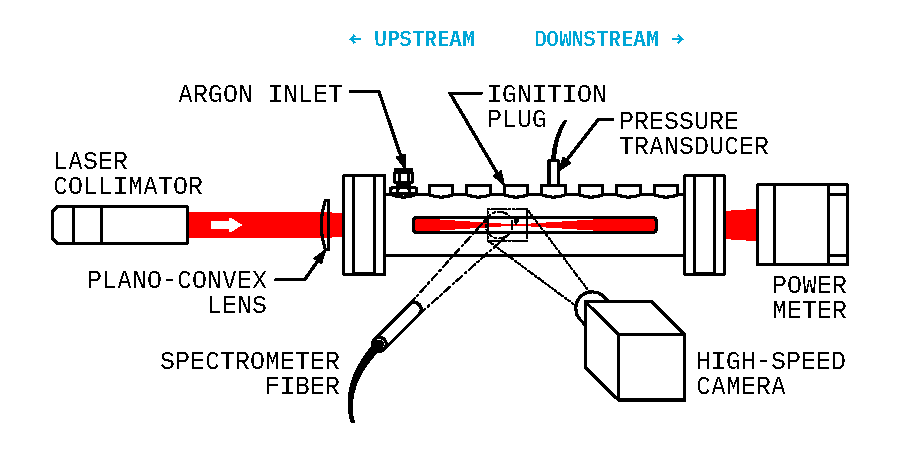
\includegraphics[width=0.85\textwidth]{assets/3 design/finalsetup_static.pdf}
                \caption{Static setup}
            \end{subfigure}
            \hfill
            \begin{subfigure}[t]{\textwidth}
                \centering
                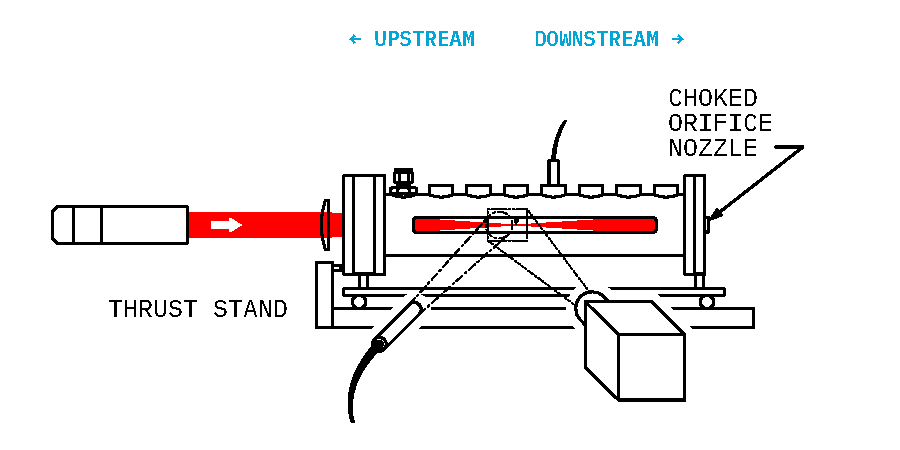
\includegraphics[width=0.85\textwidth]{assets/3 design/finalsetup_flowing.pdf}
                \caption{Flowing setup}
            \end{subfigure}
            \caption{V1 LTP thruster from \textcite{duplayArgonLaserPlasmaThruster2024a}}
            \label{fig:V1 setup}
        \end{figure}

        298 recorded pulsed laser shots were conducted with V1, exploring the power-pressure threshold, wire initiation and spark initiation. A side window permitted direct visualization of the LSP with a high speed camera (Photron Fastcam SA5).

    \section{Version 2} \label{sec:design_v2}

        To improve upon the V1 facility, an entire LTP thruster redesign was done. This resulted in the much smaller Version 2 (V2) purpose-built LTP thruster at the end of April 2024, seen in \autoref{fig:V2 render}.

        \begin{figure}[!ht]
            \centering
            \begin{subfigure}[t]{\textwidth}
                \centering
                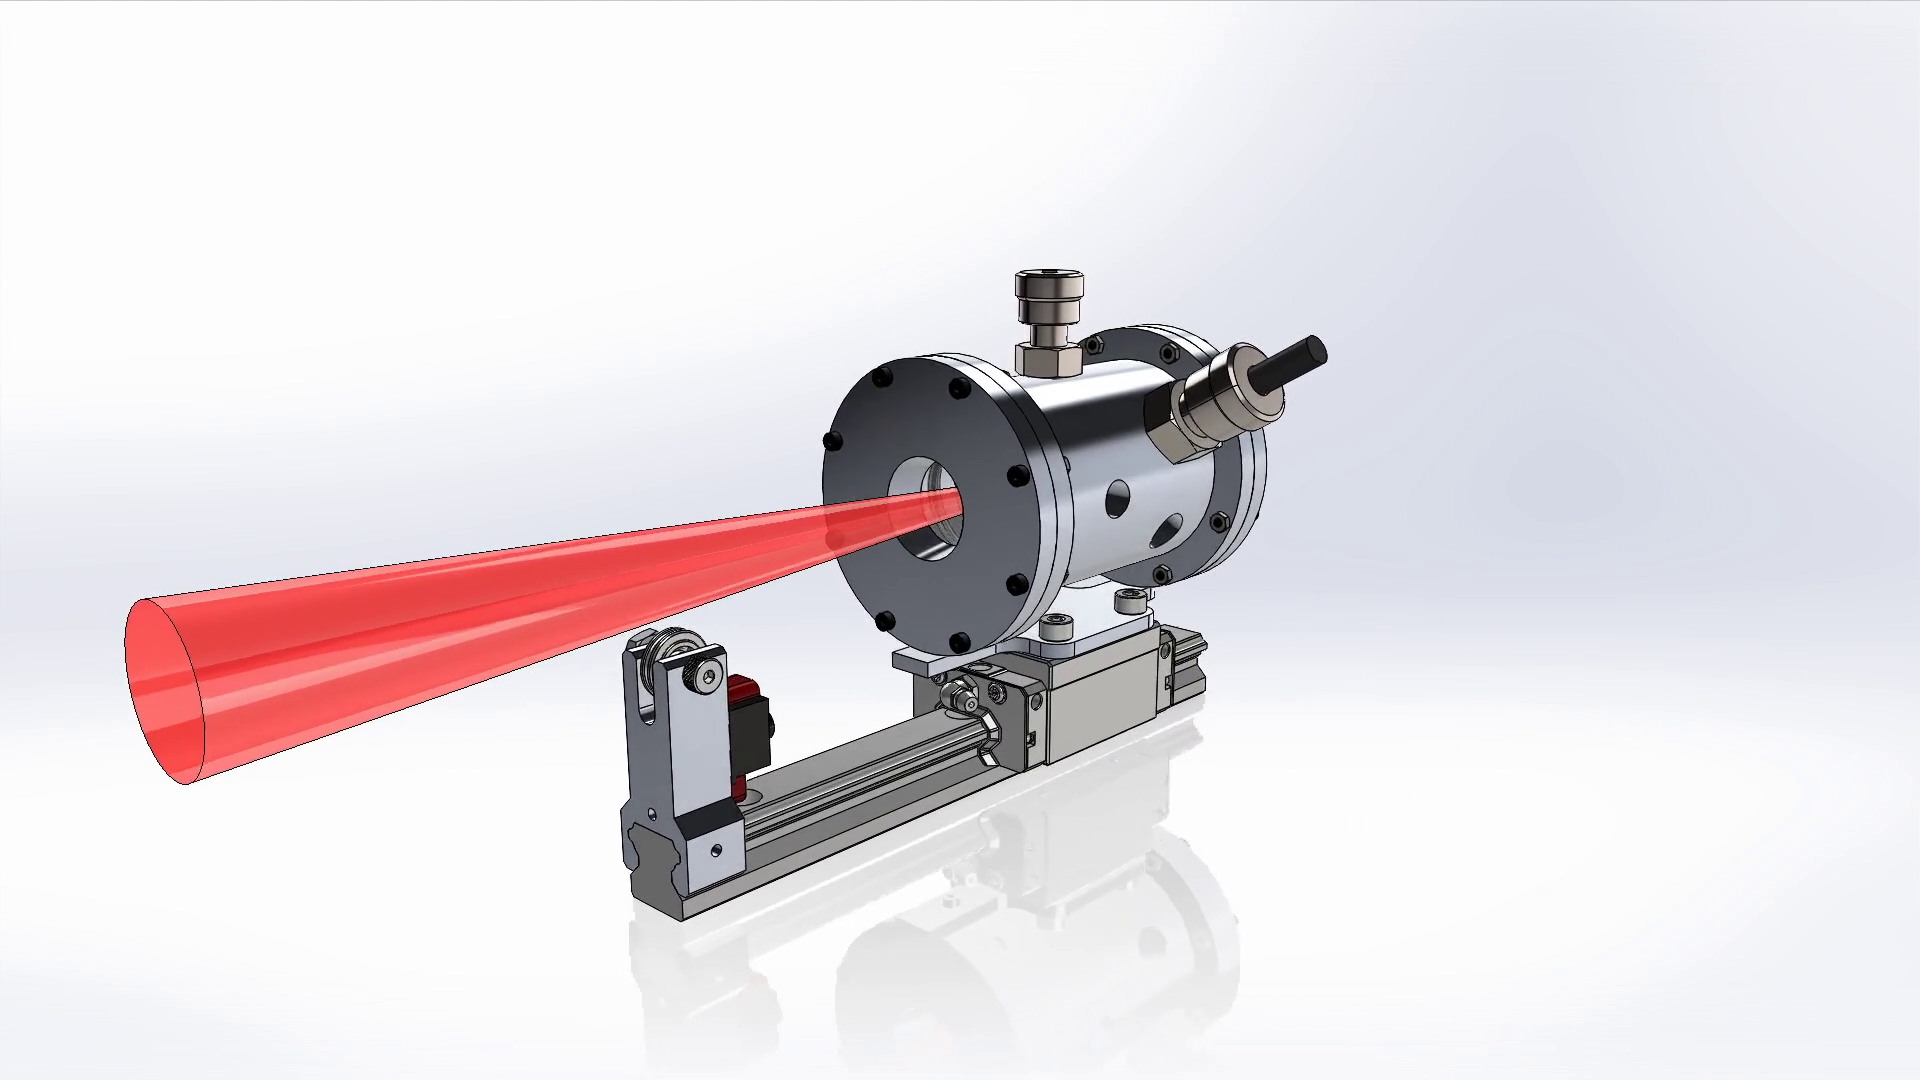
\includegraphics[width=0.85\textwidth]{assets/3 design/V2 render 45 view.png}
                \caption{View of the laser path (in red) and thruster mounted on its thrust stand}
            \end{subfigure}
            \hfill
            \begin{subfigure}[t]{\textwidth}
                \centering
                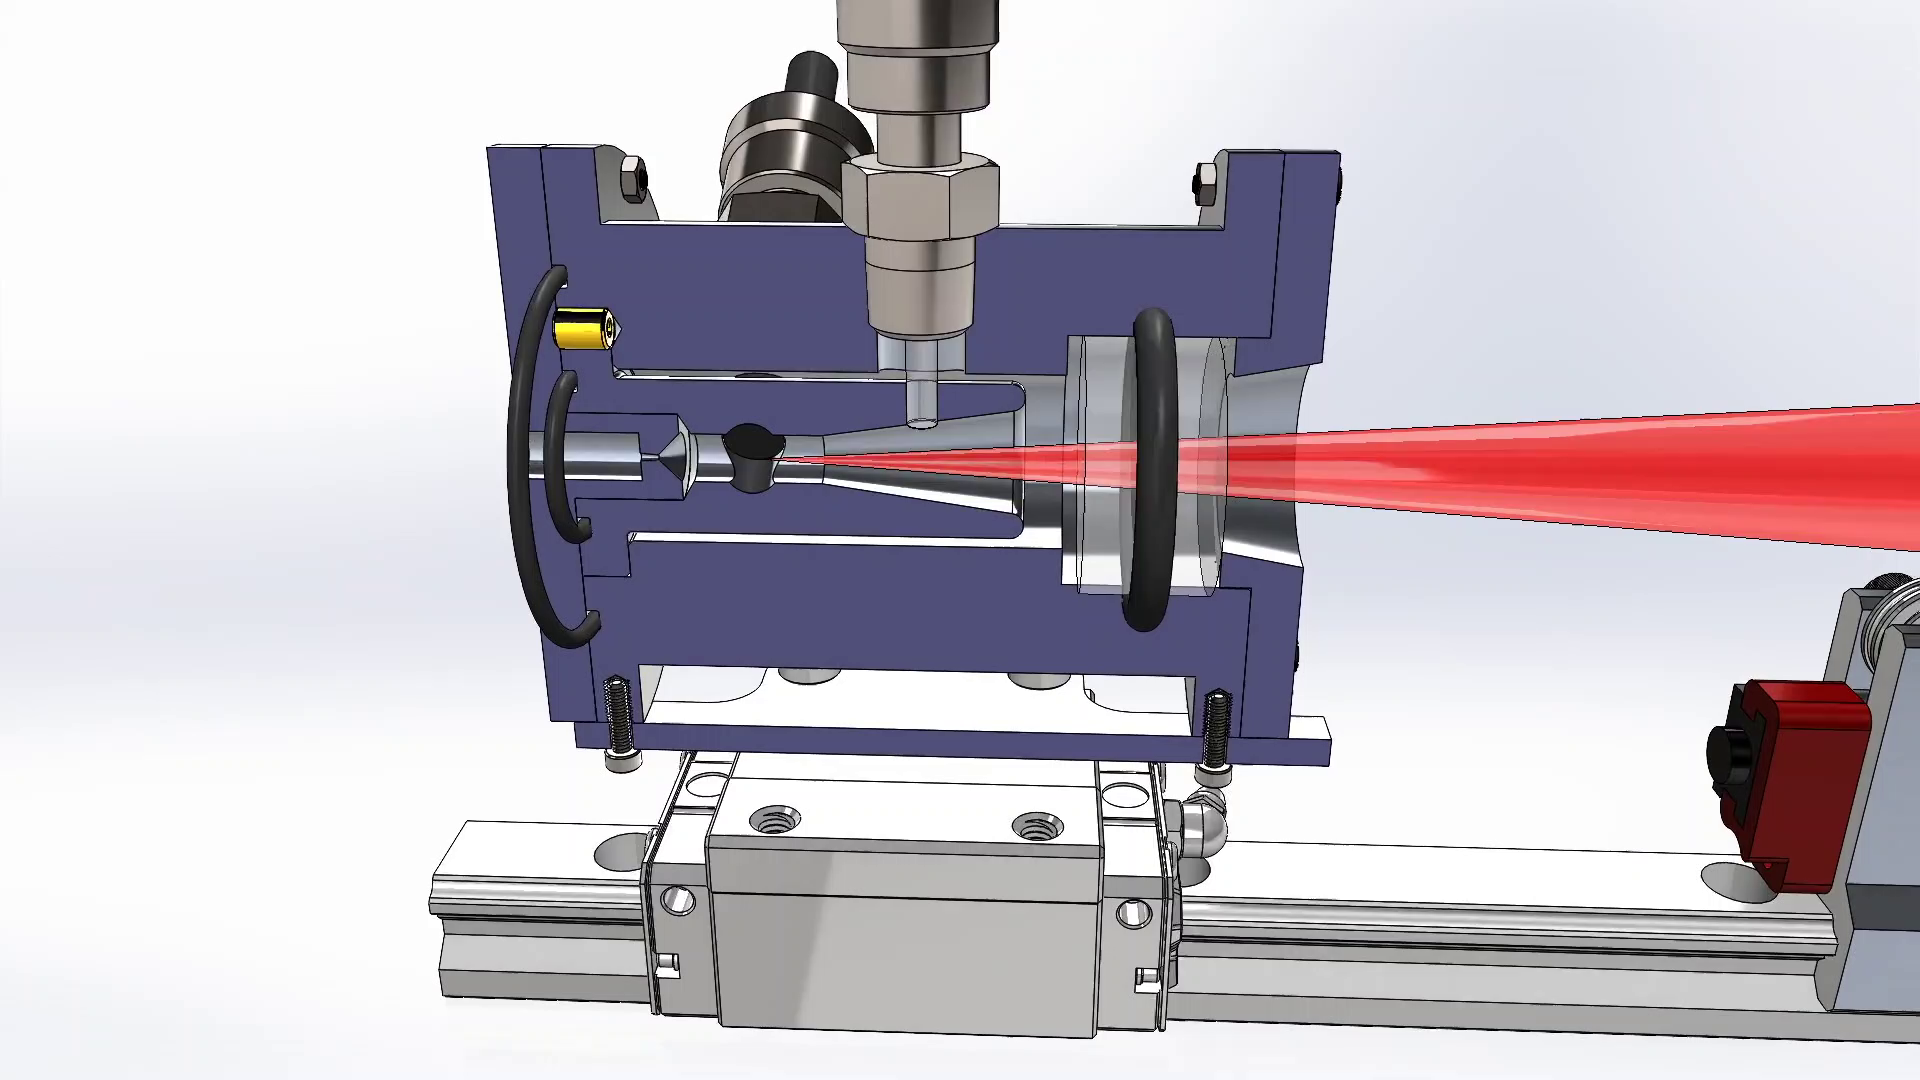
\includegraphics[width=0.85\textwidth]{assets/3 design/V2 render cutout.png}
                \caption{Cutaway view of the inside of the thruster}
            \end{subfigure}
            \caption{Render of the V2 LTP thruster}
            \label{fig:V2 render}
        \end{figure}

        \subsection{Requirements}

            The following requirements were developed for the design of the V2 thruster. The objective was to detect a measurable difference in thrust between an argon cold gas thruster and an argon “hot gas” thruster, heated by a laser supported plasma (LSP).

            \begin{enumerate}
                \item Laser thruster
                \begin{enumerate}
                    \item A \qty{300}{W} Continuous Wave (CW) \qty{1070}{nm} laser shall sustain the plasma (Nominal power \qty{300}{W}, actual max power \qty{350}{W})
                    \item The thruster shall have a minimum safe “hot” operation time of \qty{30}{s}
                    \begin{enumerate}
                        \item In the event of failed LSP initiation, the thruster shall safely absorb the total laser power for at least \qty{10}{s}
                    \end{enumerate}
                    \item An optical path shall be present to let the laser into the thruster, utilizing a \qty{100}{mm} focal length lens at minimum and a collimated beam with a maximum diameter of \qty{30}{mm}
                    \begin{enumerate}
                        \item The optical components shall not be damaged by the laser flux
                    \end{enumerate}
                    \item Argon shall be used as the working fluid
                    \begin{enumerate}
                        \item The argon feed gas shall be at room temperature
                    \end{enumerate}
                    \item A gas feed path shall bring argon gas into the thruster
                    \begin{enumerate}
                        \item The gas feed shall be choked at the thruster inlet
                        \item The gas feed shall be evenly distributed in the thruster
                    \end{enumerate}
                    \item The mass flow rate of the argon gas shall be measured and controlled by interchangeable upstream choked orifices
                    \item The maximum allowable operating pressure (MAOP) of the thruster shall be 50 bar
                    \begin{enumerate}
                        \item The nominal pressure of the thruster shall be 25 bar
                    \end{enumerate}
                    \item A converging-diverging exhaust nozzle shall be designed to accelerate the gas to a supersonic speed
                    \begin{enumerate}
                        \item The nozzle shall be easily changeable
                    \end{enumerate}
                    \item A 1/8" NPT port for a pressure transducer shall be present along the thruster
                    \item An optical port shall be present for spectrometry measurements of the plasma
                    \item The thruster shall be installed on a thrust stand (See section 3. Thrust stand)
                \end{enumerate}
                \item Initiation system/electrical
                \begin{enumerate}
                    \item The LSP shall be initiated by an electrical spark
                    \item The spark gap shall be measurable, controllable, and repeatable
                    \item The spark shall be generated by an AEM 30-2853 High Output Smart Coil, supplying \qty{41}{kV} with up to \qty{118}{mJ}
                    \item All parts of the thruster and thrust stand shall be directly or indirectly connected to a common electrical ground
                \end{enumerate}
                \item Thrust stand
                \begin{enumerate}
                    \item The thrust stand shall measure thrust on the order of \qtyrange{0.1}{5}{N}
                    \item The thrust stand shall minimize friction losses
                    \item The thrust stand shall be securely fixed using standard optical breadboard mounting hardware
                \end{enumerate}
            \end{enumerate}

            With these requirements, preliminary geometric dimensions of the V2 thruster could commence. It was expected to be much smaller than V1, as the goal was to isolate the LSP region and increase heat flux to the gas.

        \subsection{Initial sizing of the double choked LTP thruster}

            When adding energy to the thruster chamber with a laser, it is useful to choke the inflow upstream of the chamber. Indeed, this keeps the $P_0$ and $\dot{m}_\mathrm{in}$ constant, so the increase in chamber pressure can be interpreted as a measure of energy deposition. The second choke happens at the nozzle to accelerate the hot gas to a supersonic speed. Therefore, this configuration is double choked (see \autoref{fig:double choke sizing}), a classic problem in compressible fluid mechanics.

            \begin{figure}[h]
                \centering
                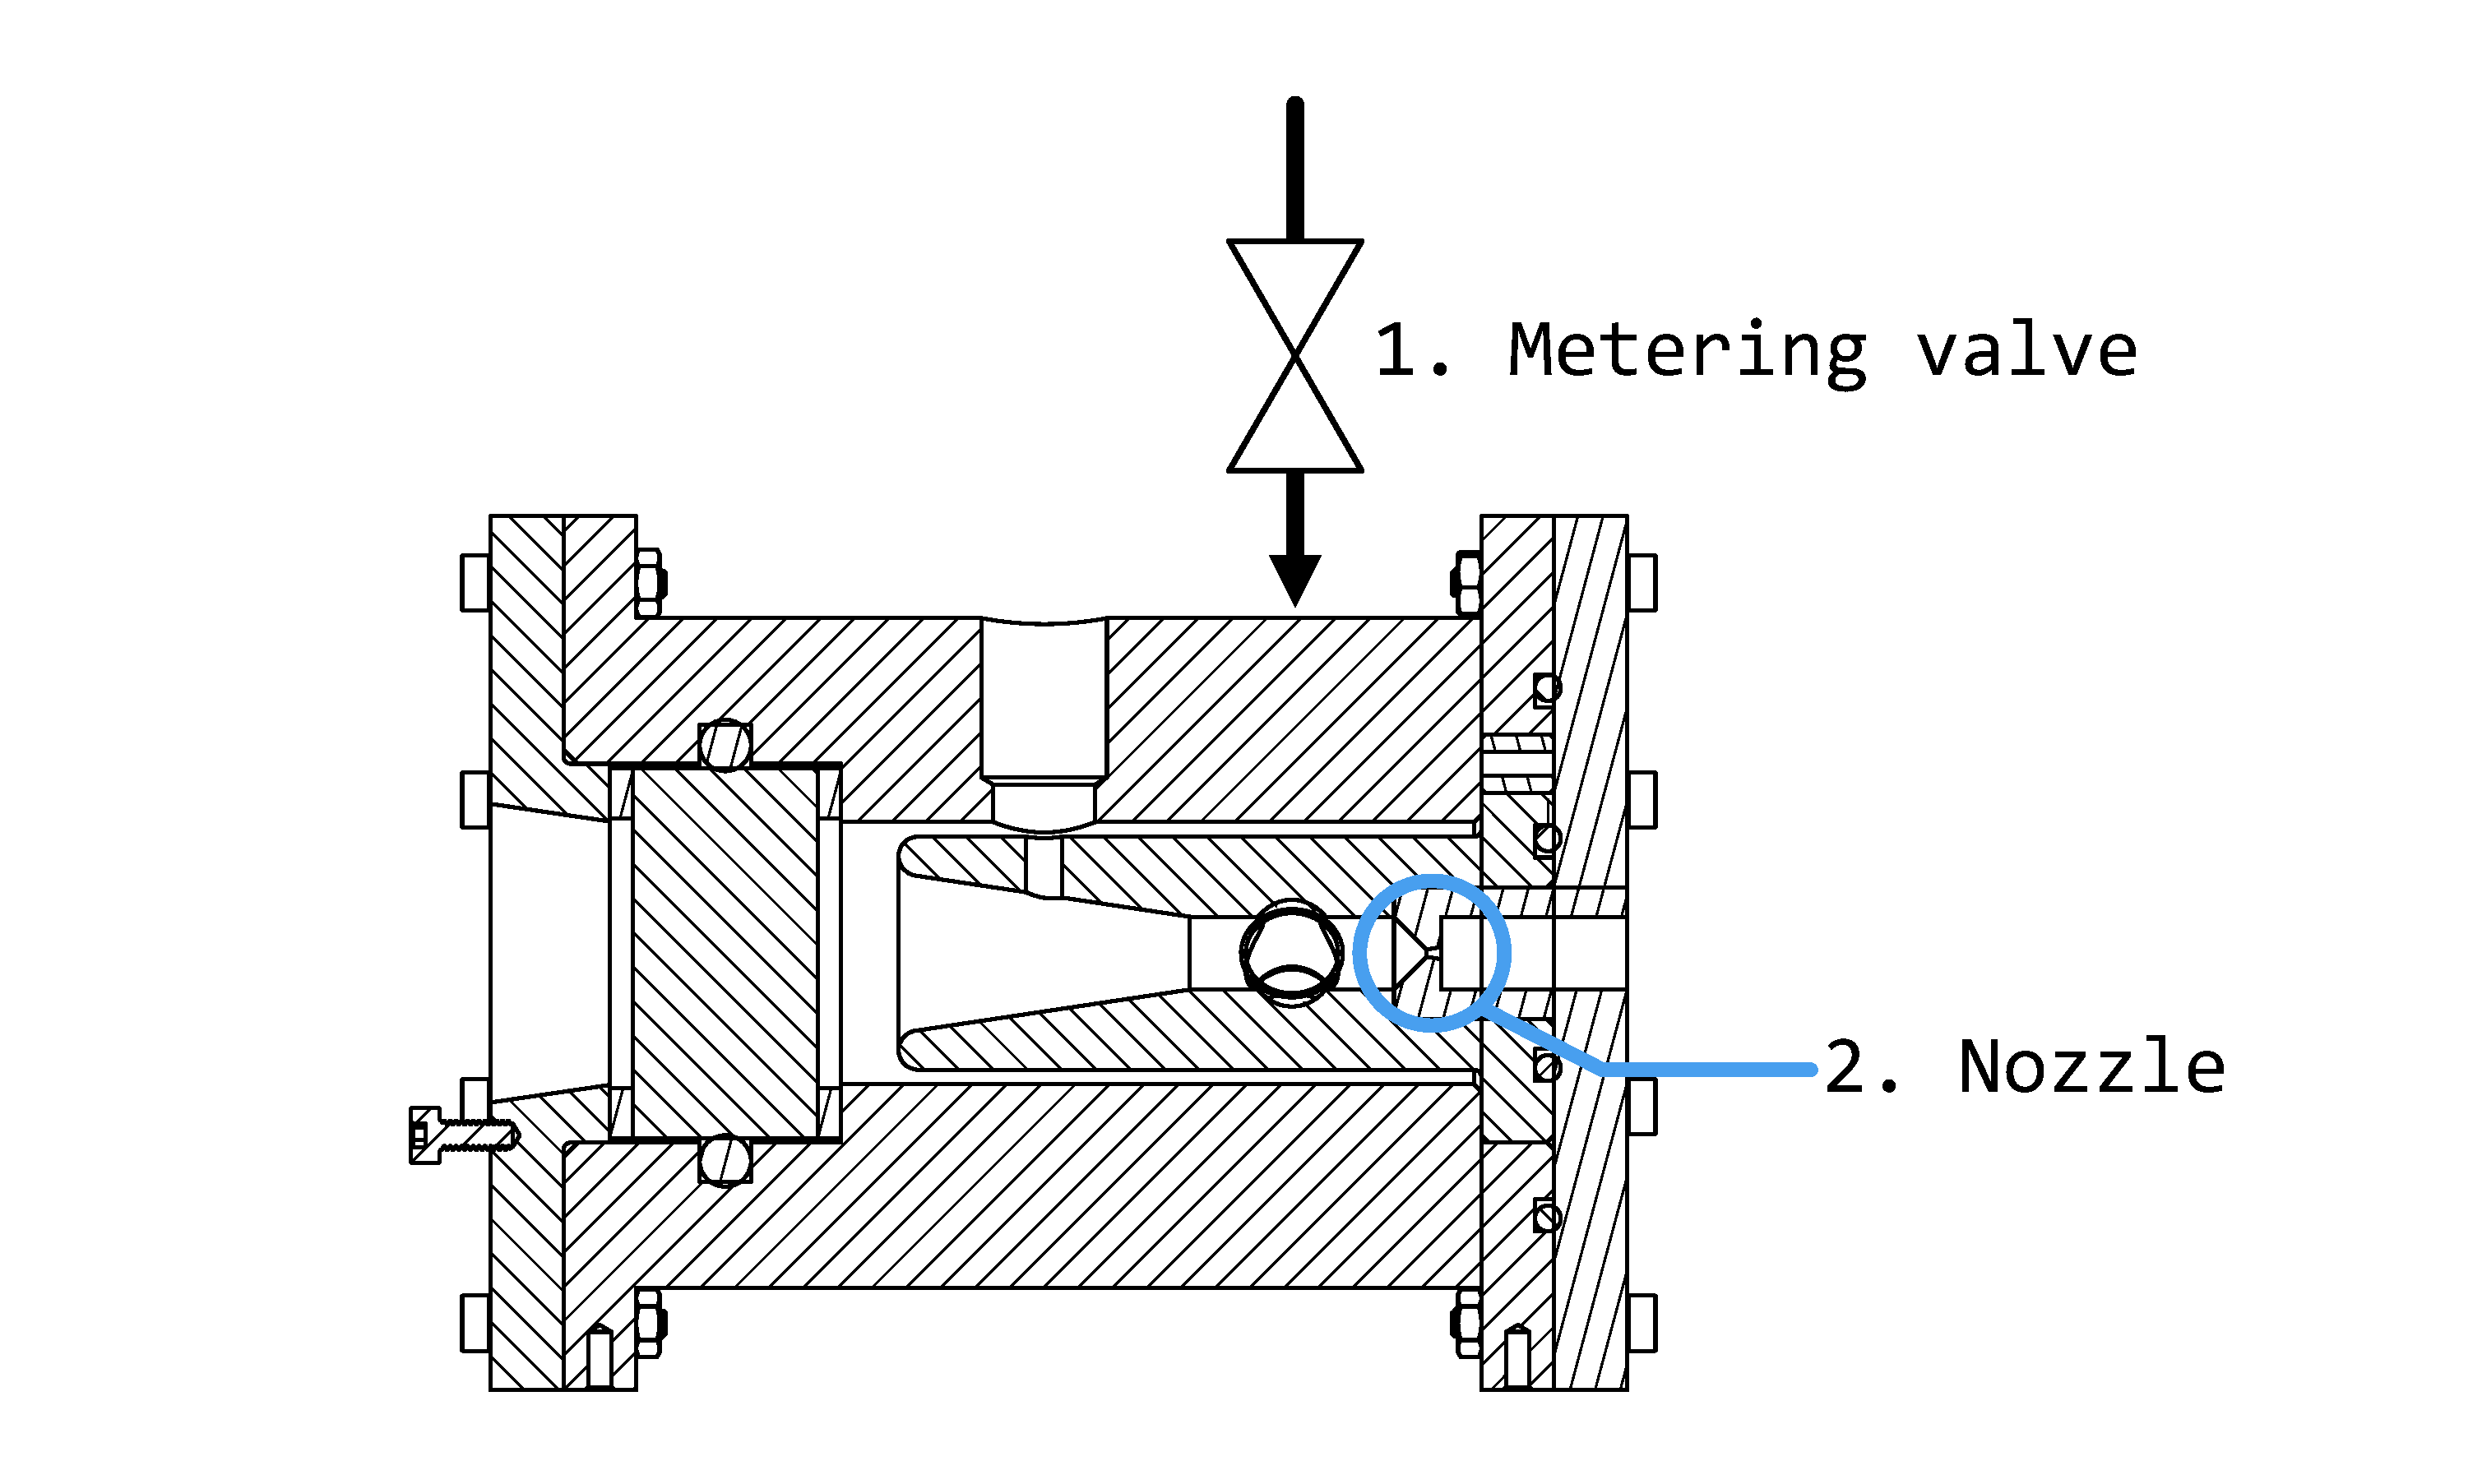
\includegraphics[width=0.8\linewidth]{assets/3 design/Double choked LTP thruster.pdf}
                \caption{Cutaway of a double choked LTP thruster showing both choking orifices: the metering valve and the nozzle.}
                \label{fig:double choke sizing}
            \end{figure}
            
            The starting assumptions were the following: a \qty{300}{W} power input (the laser) supplies energy to an LTP experiment that has an internal pressure of \qty{25}{bar}, with a \qty{50}{bar} feed pressure. It is required that the hot gas operation (laser on) increases the gas' exit velocity to twice that of the cold gas operation (laser off). The gas mass flow rate and the diameter of the two orifices needed to choke the flow will be determined.

            Starting with a cold gas thruster using argon, the speed of sound of argon ($c_0$) is \qty{323}{m/s}. This is at ambient temperature (\qty{300}{K}), as we have no laser energy to heat the gas in this case. With a nozzle, the gas is accelerated to approximately twice this speed. The exit velocity of the gas $v_\mathrm{exit}$, which is our main performance parameter, is therefore \qty{646}{m/s}.
            
            Laser on (hot) operation will now be examined. Taking the previous $v_\mathrm{exit}$ and ionizing the whole flow, it is assumed that the thruster's efficiency is doubled. This gives a $v_\mathrm{exit}\approx \qty{1300}{m/s}$. What nozzle throat size is therefore necessary for this $\dot m$ with $p_\mathrm{chamber} = \qty{25}{bar}$? $\mathrm{MW_{Ar}} = \qty{40}{g/mol}$ and the speed of sound is $c = \sqrt{\gamma R T}$. As the speed of sound will be doubled, the temperature is multiplied by 4.
            \[\text{Power} = \dot m (h_2-h_1)
            = \dot m c_p (T_2-T_1)\]
            Using a constant $c_p$ of argon of \qty{0.520}{kJ.kg^{-1}.K^{-1}}, the calculated $\dot m$ is \qty{0.641}{g/s}. Fliegner's formula describes the mass flow rate of an isentropic flow:
            \[\frac{\dot m}{A} = p_0\sqrt{\frac{\gamma}{T_0 R}}\frac{M}{(1+\frac{\gamma-1}{2}M^2)^{(\frac{\gamma+1}{2(\gamma-1)})}}\]
            With $\gamma = \frac{c_p}{c_v} = 1.67$ for argon and choked flow at the nozzle, the area and the diameter of the circular nozzle are \qty{0.176}{mm^2} and \qty{0.473}{mm}, respectively. The V2 test section was built with this nozzle diameter. These calculations can be repeated for the feed orifice, with the same $\dot m$, a pressure of \qty{50}{bar} and ambient temperature. This gives us an orifice diameter of about 0.2 mm.
        
        \subsection{Test section and thrust stand}
            
            As can be seen in \autoref{fig:V2 setup}, the V2 test section was designed with multiple ports for modularity, enabling static and flowing tests with argon propellant. Ports that were not in use were fitted with pipe plugs. In all tests, the two opposing electrode ports and one argon inlet port were used. The second argon inlet, intended to offer a more uniform flow if needed, was not used. The optical access port was initially fitted with a quartz rod in an Ultra-Torr fitting. After flowing through the test section, used argon propellant was vented directly to the lab. \autoref{fig:V2 IRL setup} shows the two final configurations in the lab.

            \begin{figure}[!ht]
                \centering
                \begin{subfigure}[t]{\textwidth}
                    \centering
                    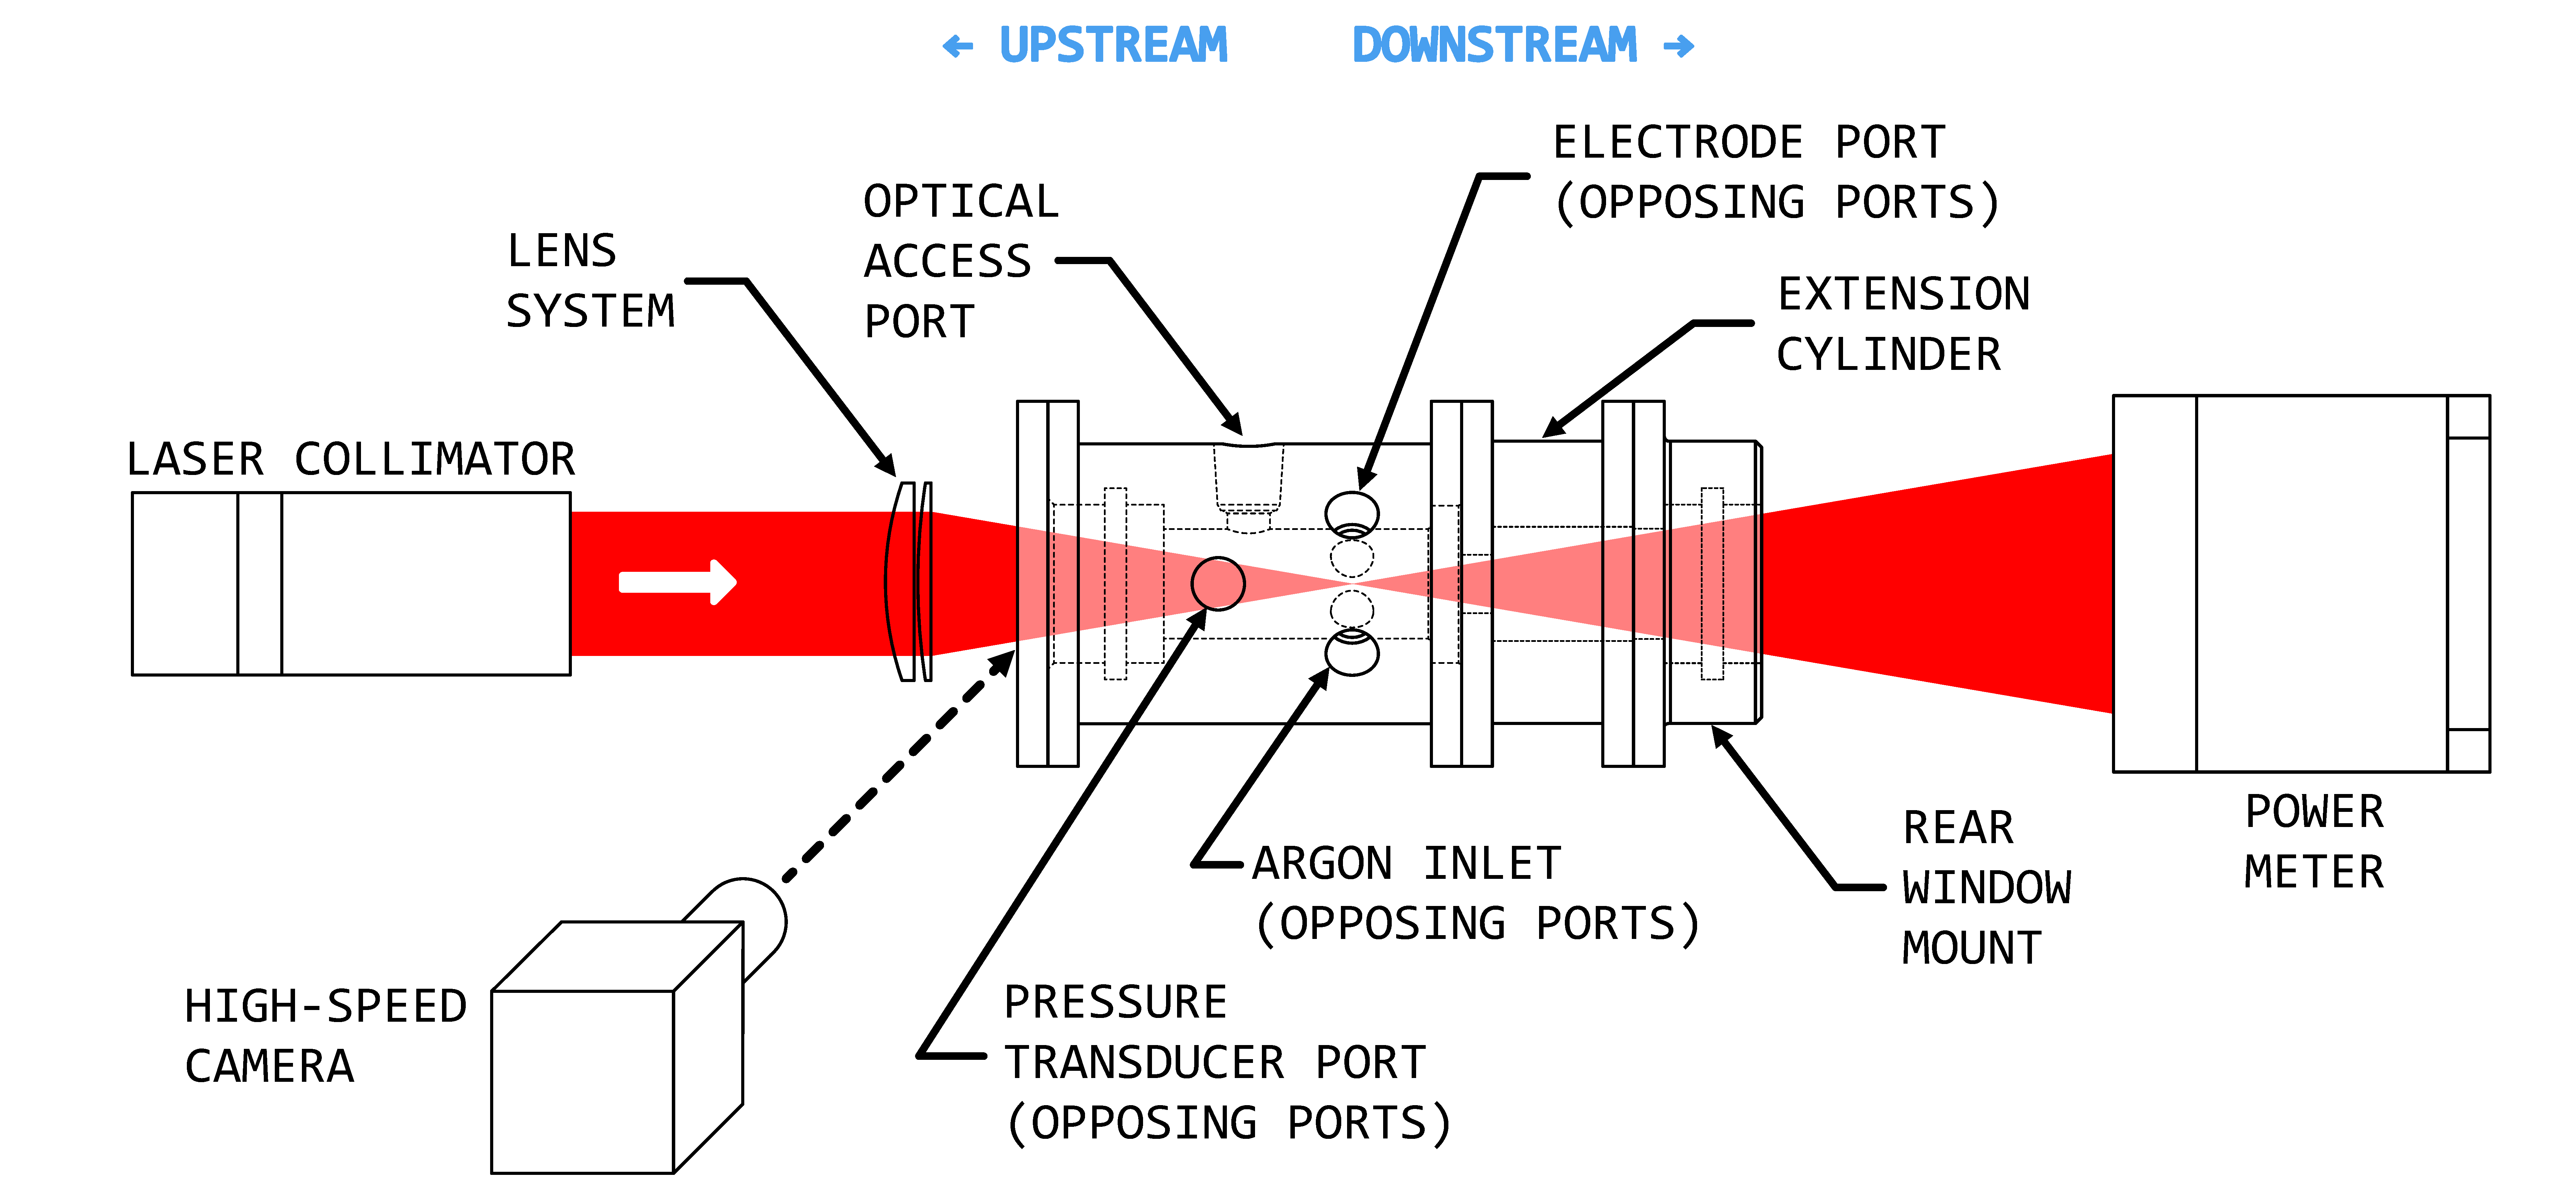
\includegraphics[width=0.85\textwidth]{assets/3 design/V2 Static config.pdf}
                    \caption{Static configuration}
                \end{subfigure}
                \hfill
                \begin{subfigure}[t]{\textwidth}
                    \centering
                    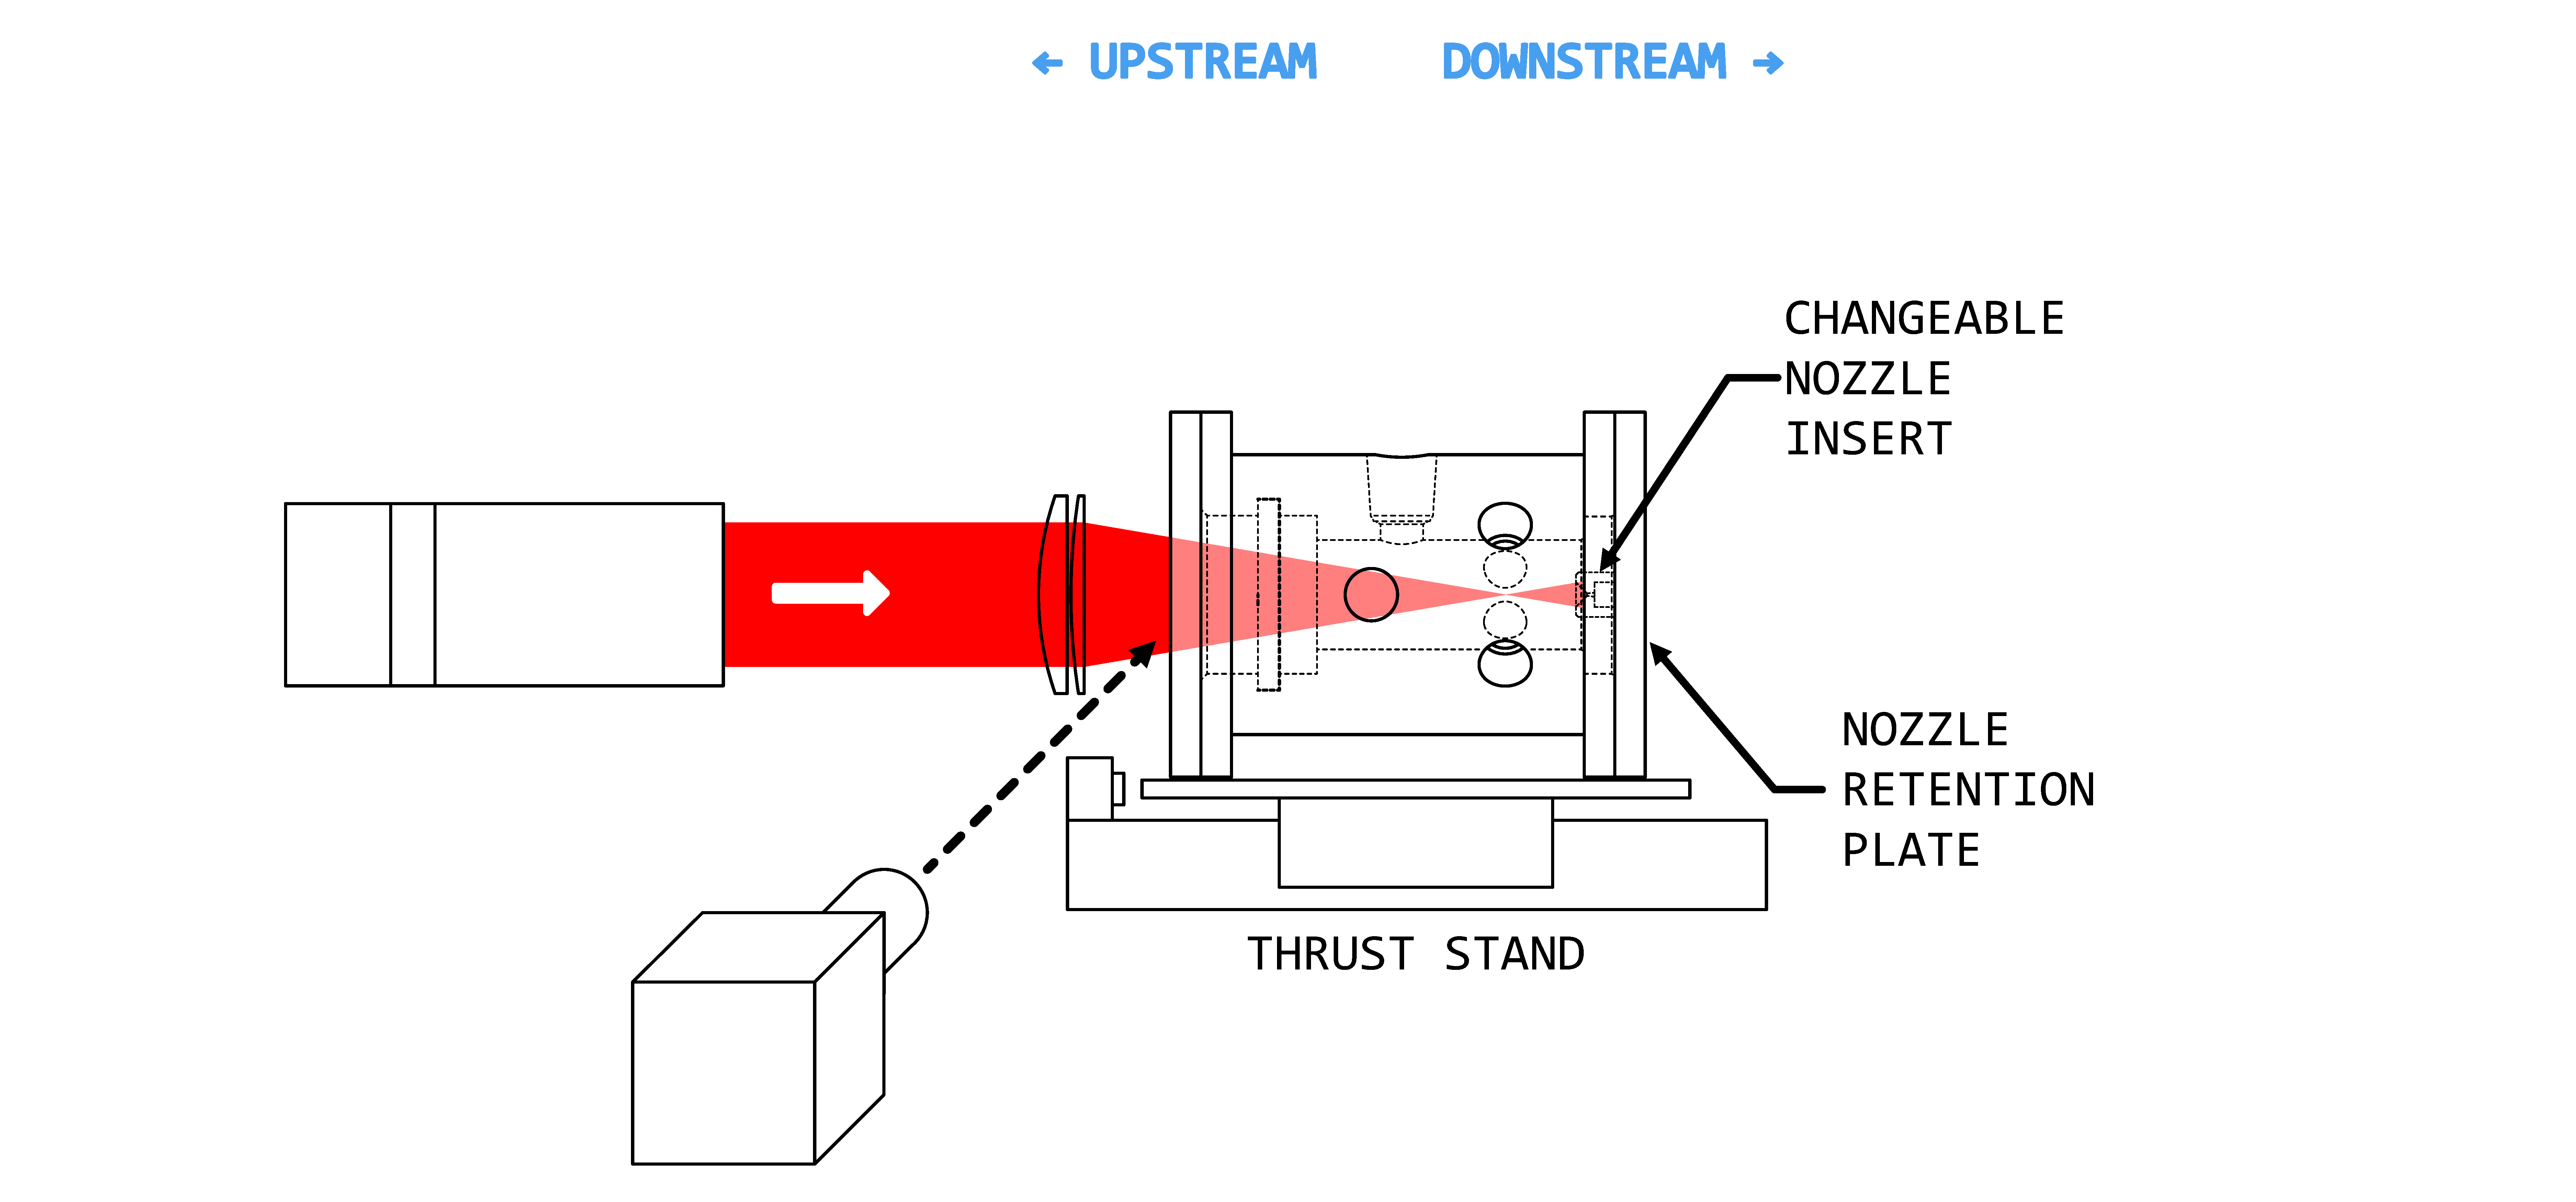
\includegraphics[width=0.85\textwidth]{assets/3 design/V2 Flowing config.pdf}
                    \caption{Flowing configuration}
                \end{subfigure}
                \caption{V2 LTP thruster}
                \label{fig:V2 setup}
            \end{figure}

            \begin{figure}[!ht]
                \centering
                \begin{subfigure}[t]{0.45\textwidth}
                    \centering
                    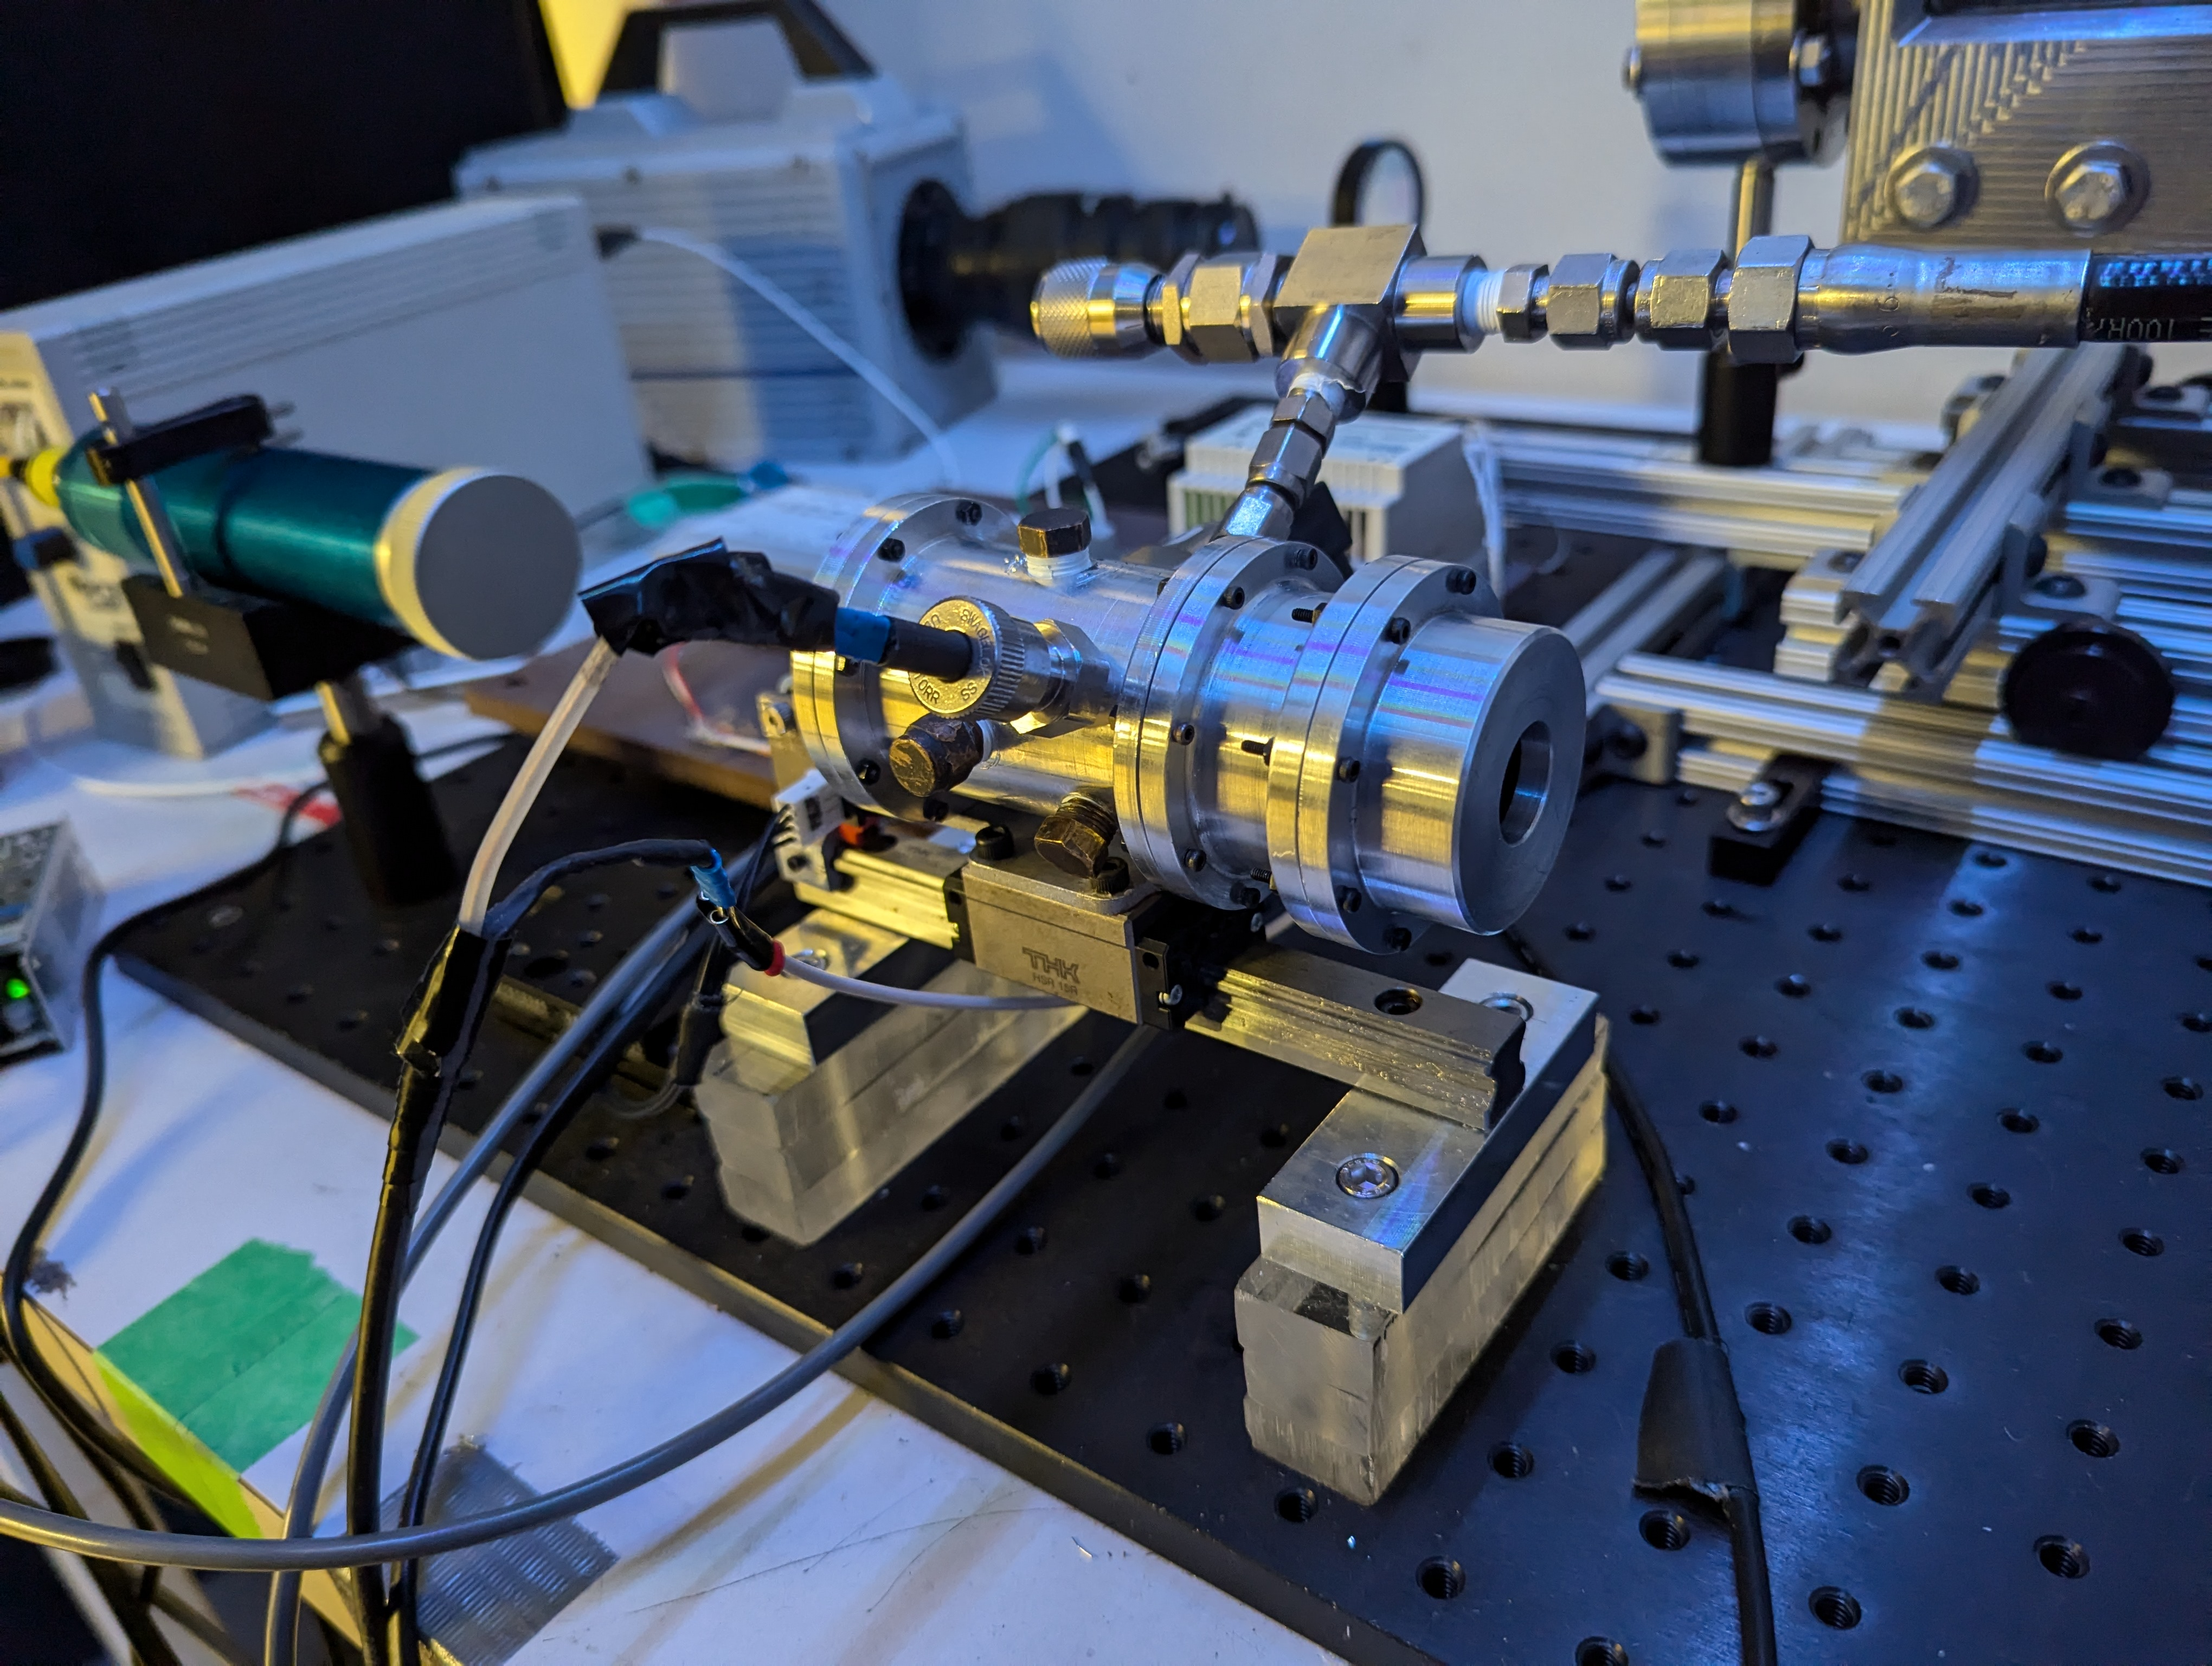
\includegraphics[width=\textwidth]{assets/3 design/V2 Static configuration.jpg}
                    \caption{Final static configuration. Note the extension part and window mount. Optics and laser collimator are not pictured here, but would be installed during testing.}
                \end{subfigure}
                \hfill
                \begin{subfigure}[t]{0.45\textwidth}
                    \centering
                    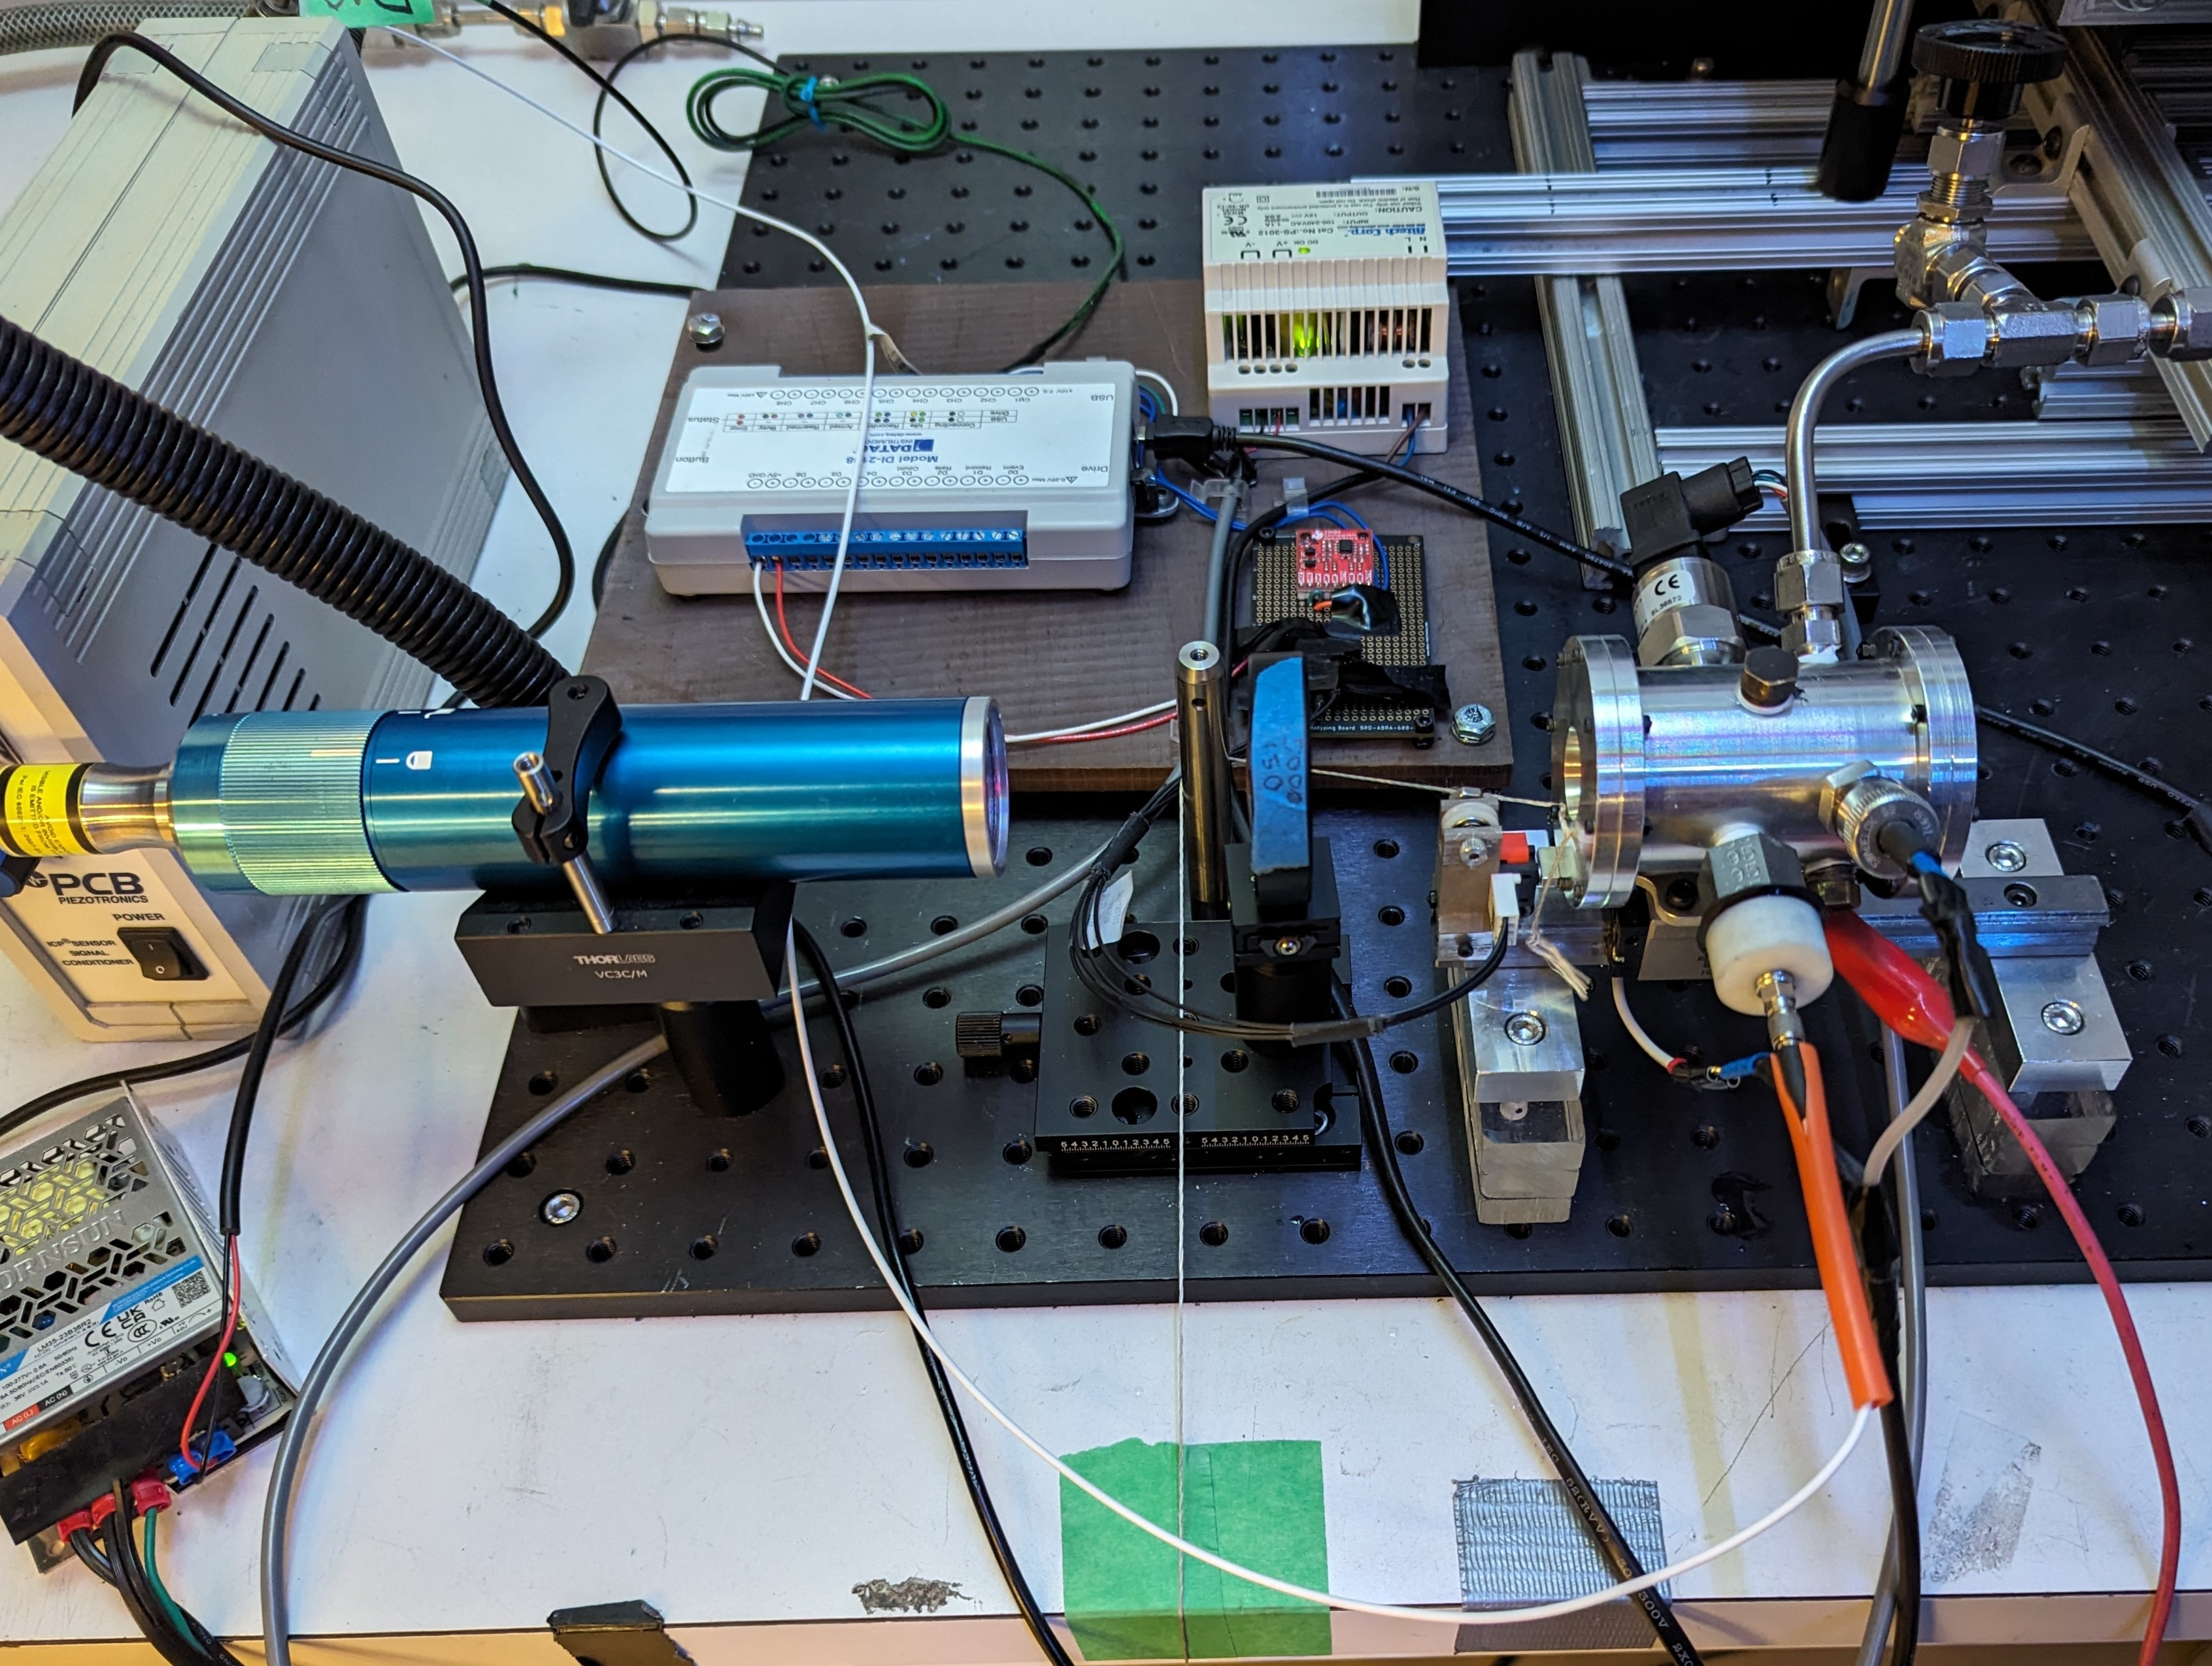
\includegraphics[width=\textwidth]{assets/3 design/V2 flowing setup.jpg}
                    \caption{Final flowing configuration. The nozzle is held by the rear plate.}
                \end{subfigure}
                \caption{V2 LTP thruster}
                \label{fig:V2 IRL setup}
            \end{figure}

            The thrust stand is a ball bearing carriage (McMaster-Carr 6709K12) on a \qty{15}{mm} wide, \qty{160}{mm} long guide rail (McMaster-Carr 6709K33). The rail is mounted on the optical breadboard using acrylic spacers. A string through a pulley holds a variable weight, adding a preload to the test section. This ensures adequate contact between the test section and the load cell, and allows calibration of the load cell. Two load cells are used with different force sensing range: Honeywell FSG020WNPB (\qtyrange{0}{20}{N}) and Honeywell FSG005WNPB (\qtyrange{0}{5}{N}).

        \subsection{Laser and optics}

            The laser used as the plasma's power source is an IPG Photonics YLR-300/3000-QCW-MM-AC Ytterbium fiber laser. The wavelength of the emitted light is \qty{1070}{nm}. Its nominal maximum power is \qty{3}{kW} quasi-continuous wave (QCW) or \qty{300}{W} continuous wave (CW). At \qty{3}{kW}, a QCW pulse has a maximum duration of \qty{10}{ms}. The maximum duration of a \qty{300}{W} QCW pulse is \qty{50}{ms}. The IPG Photonics P30-001736 collimator outputs a \qty{30}{mm} diameter laser beam. The laser also includes a red visible laser for alignment, which is coaxial to the main beam. These components form the laser system, presented in \autoref{fig:laser and collimator}.

            \begin{figure}[!ht]
                \centering
                \begin{subfigure}[t]{0.45\textwidth}
                    \centering
                    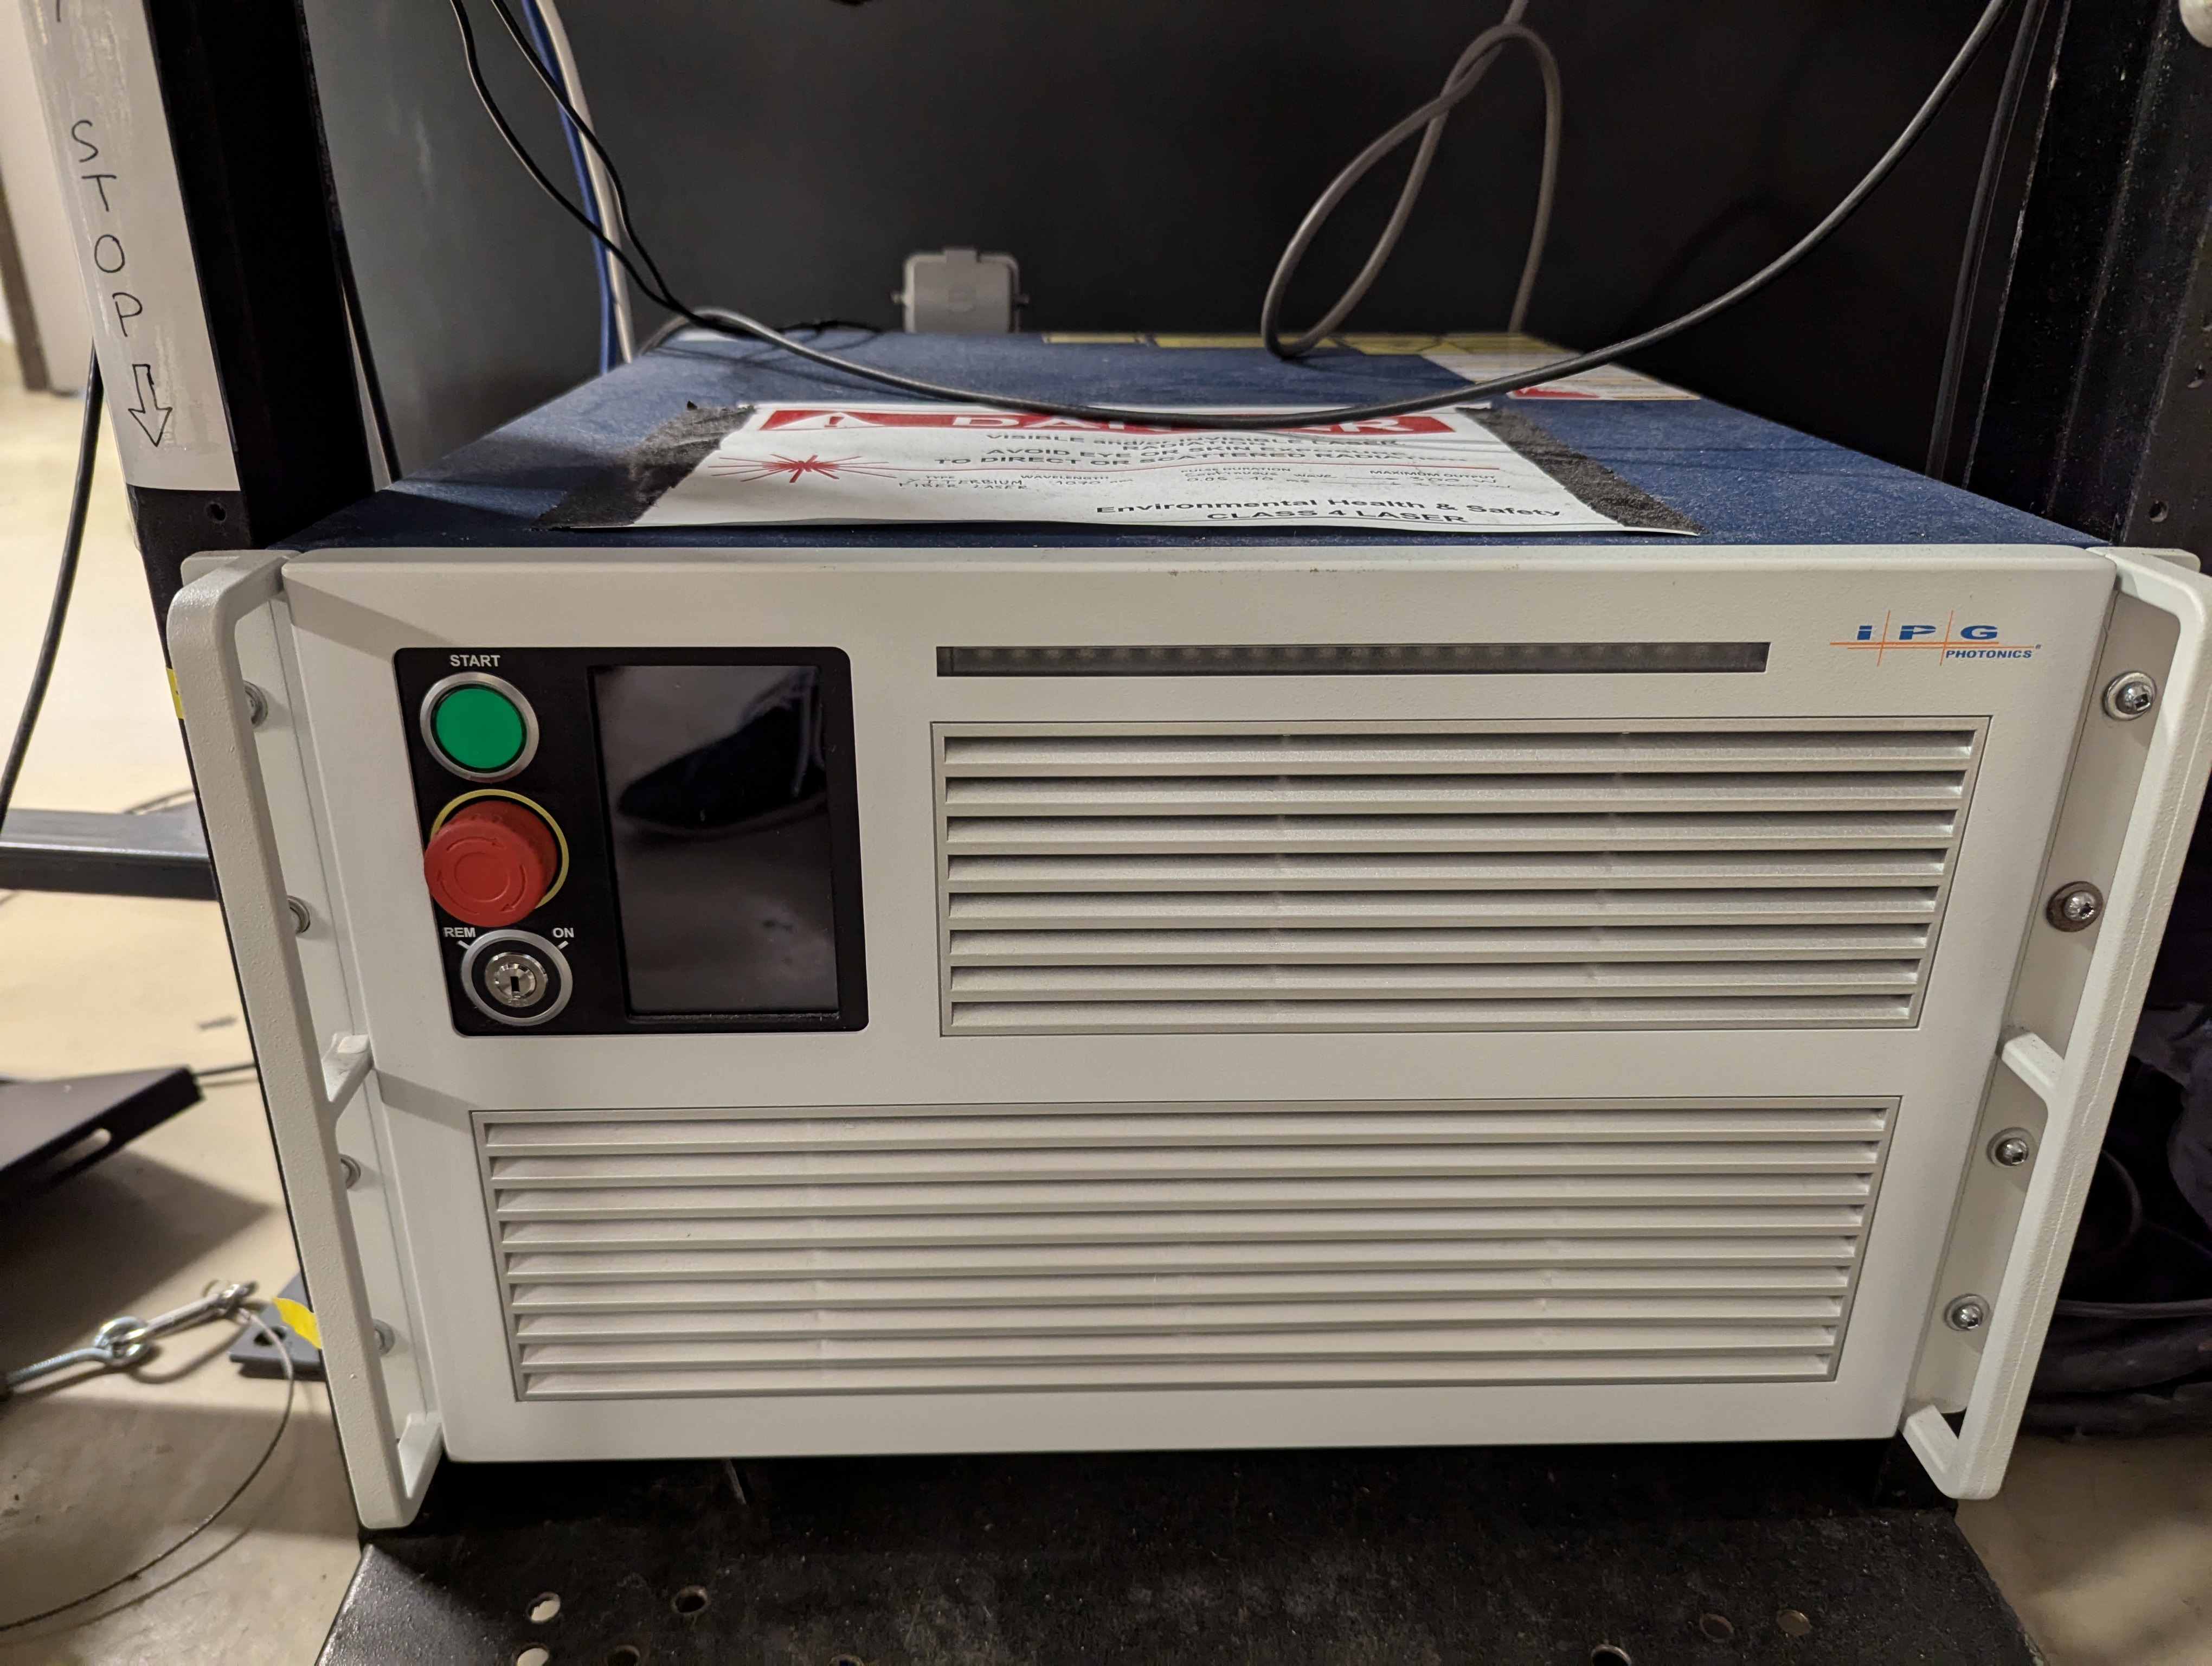
\includegraphics[width=\textwidth]{assets/3 design/Laser box.jpg}
                    \caption{IPG Photonics YLR-300/3000-QCW-MM-AC laser}
                \end{subfigure}
                \hfill
                \begin{subfigure}[t]{0.45\textwidth}
                    \centering
                    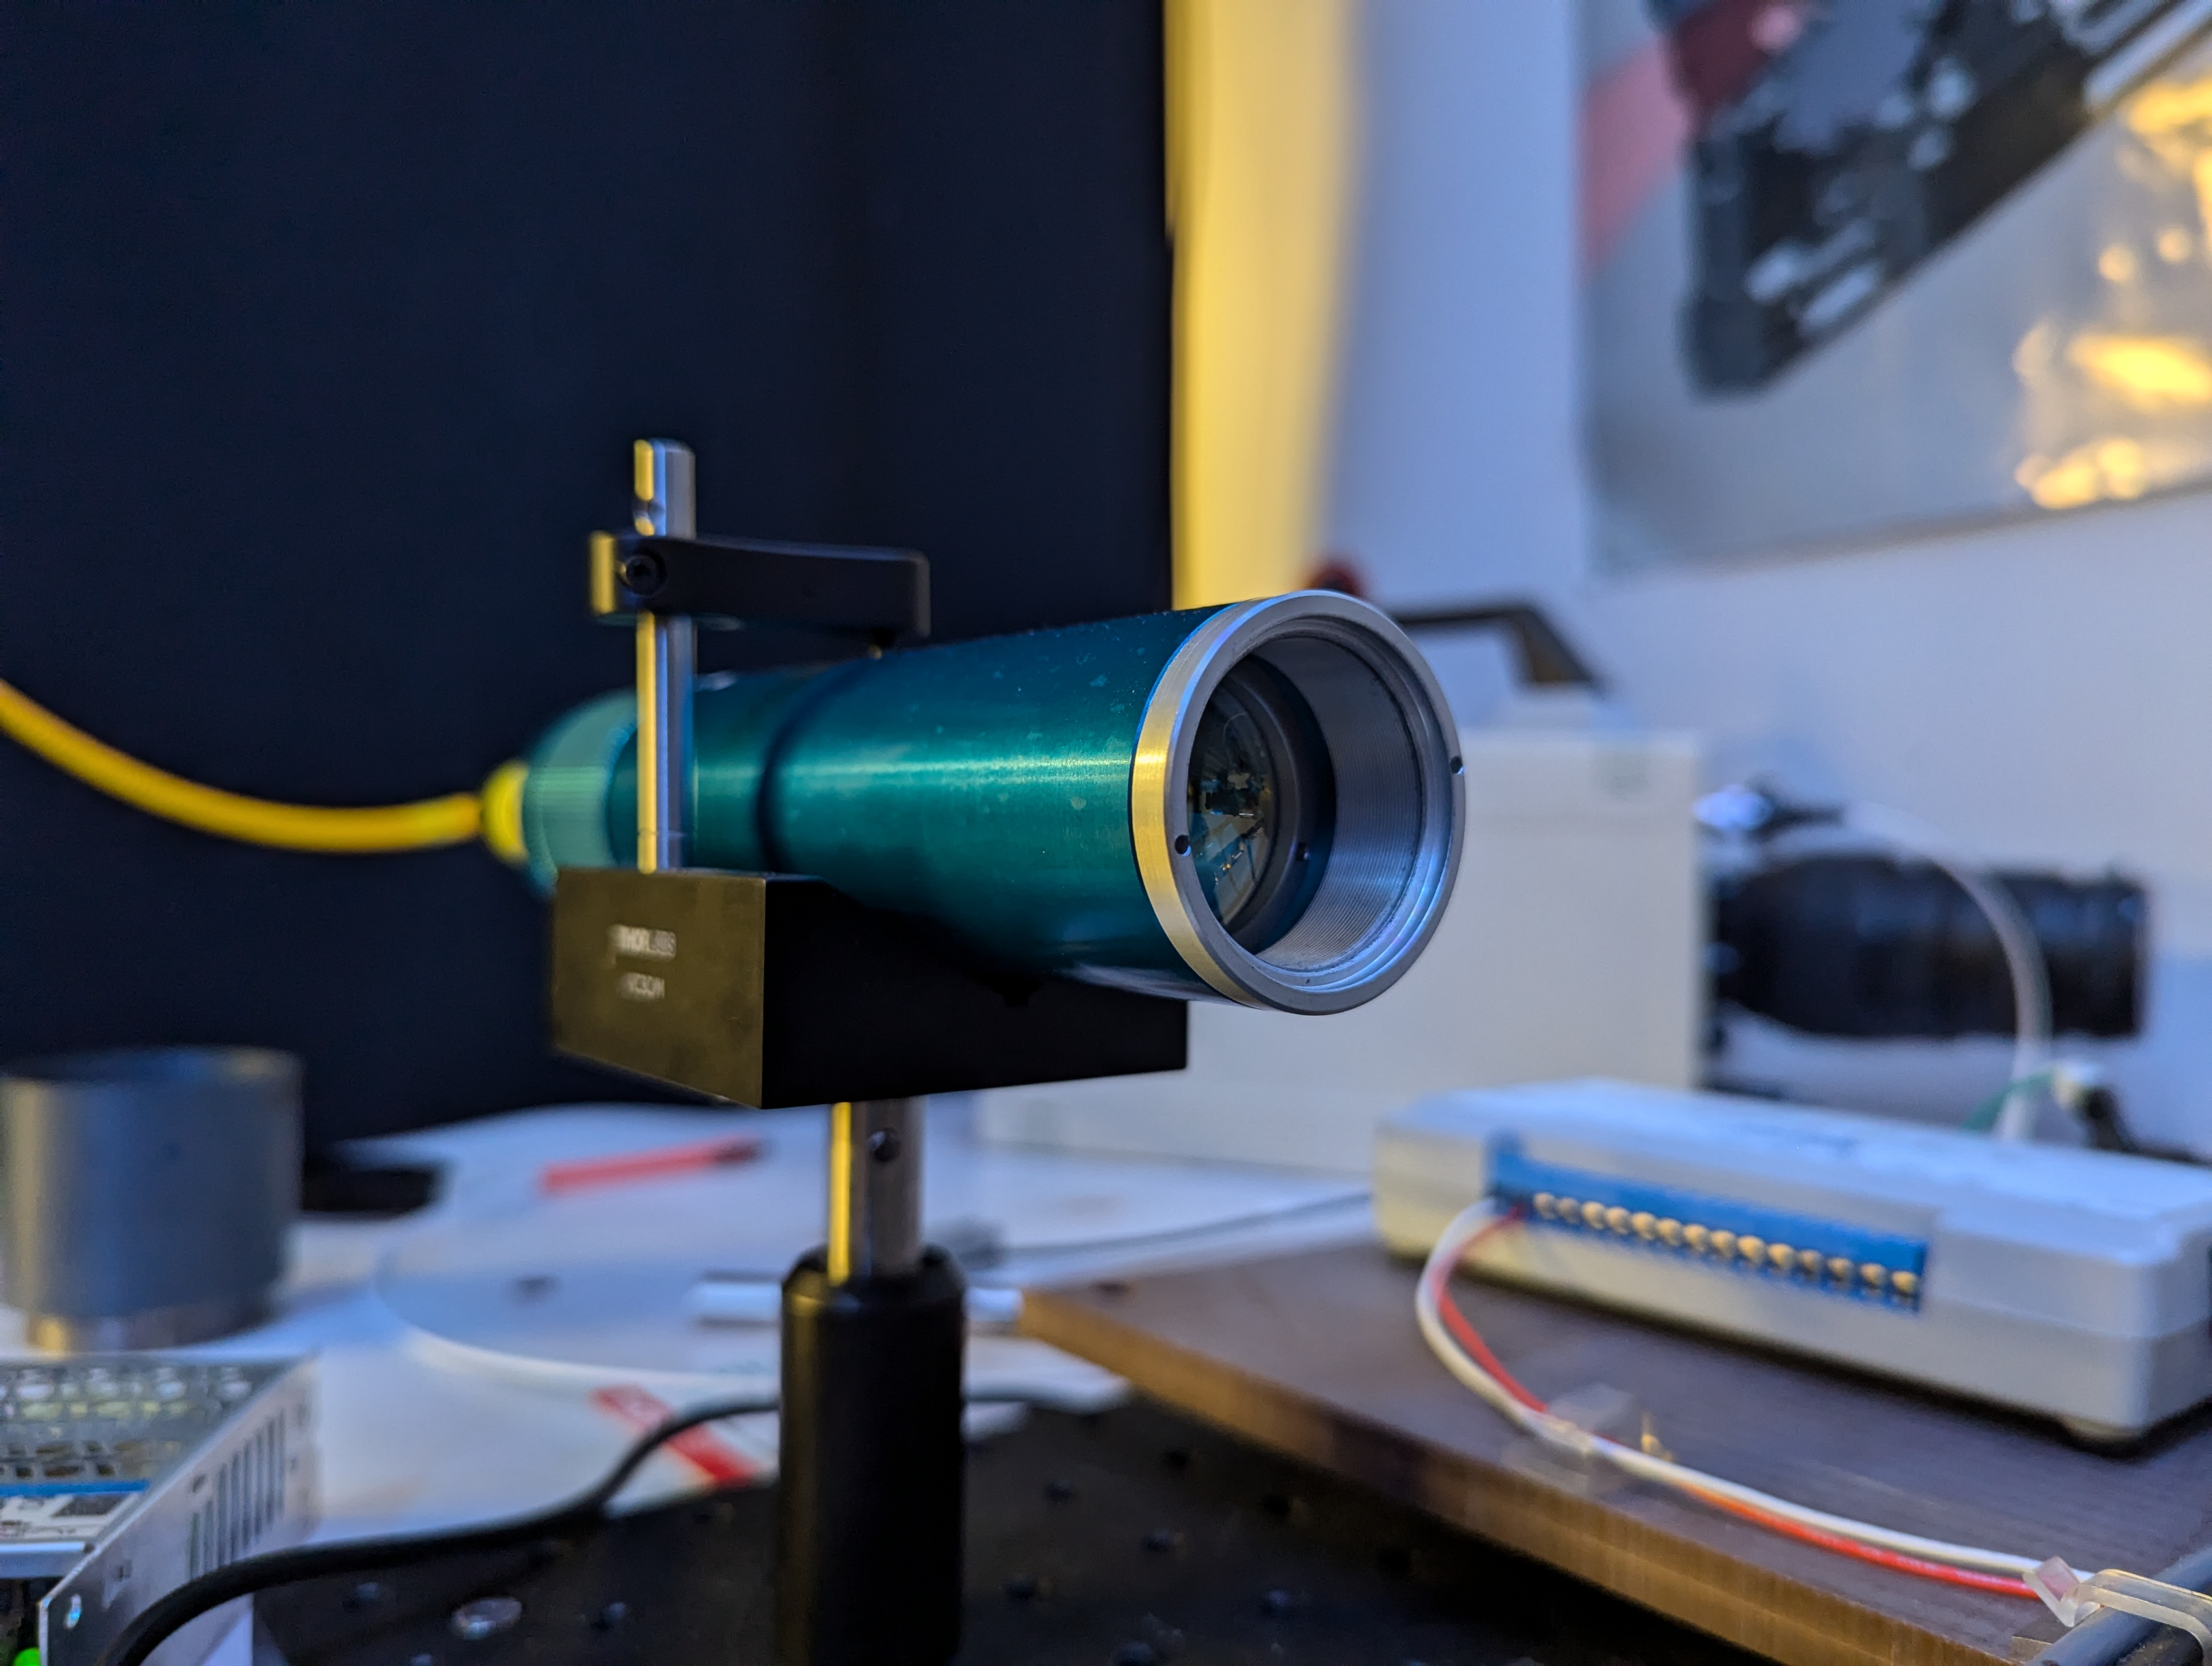
\includegraphics[width=\textwidth]{assets/3 design/Laser aperture.jpg}
                    \caption{IPG Photonics P30-001736 collimator}
                \end{subfigure}
                \caption{Laser system}
                \label{fig:laser and collimator}
            \end{figure}

            Calibration reports for the laser and the collimator can be found in \autoref{chp:app_YLR}. The laser is mounted at the base of a freestanding electronics rack (\autoref{fig:electronics rack}).

            \begin{figure}[!ht]
                \centering
                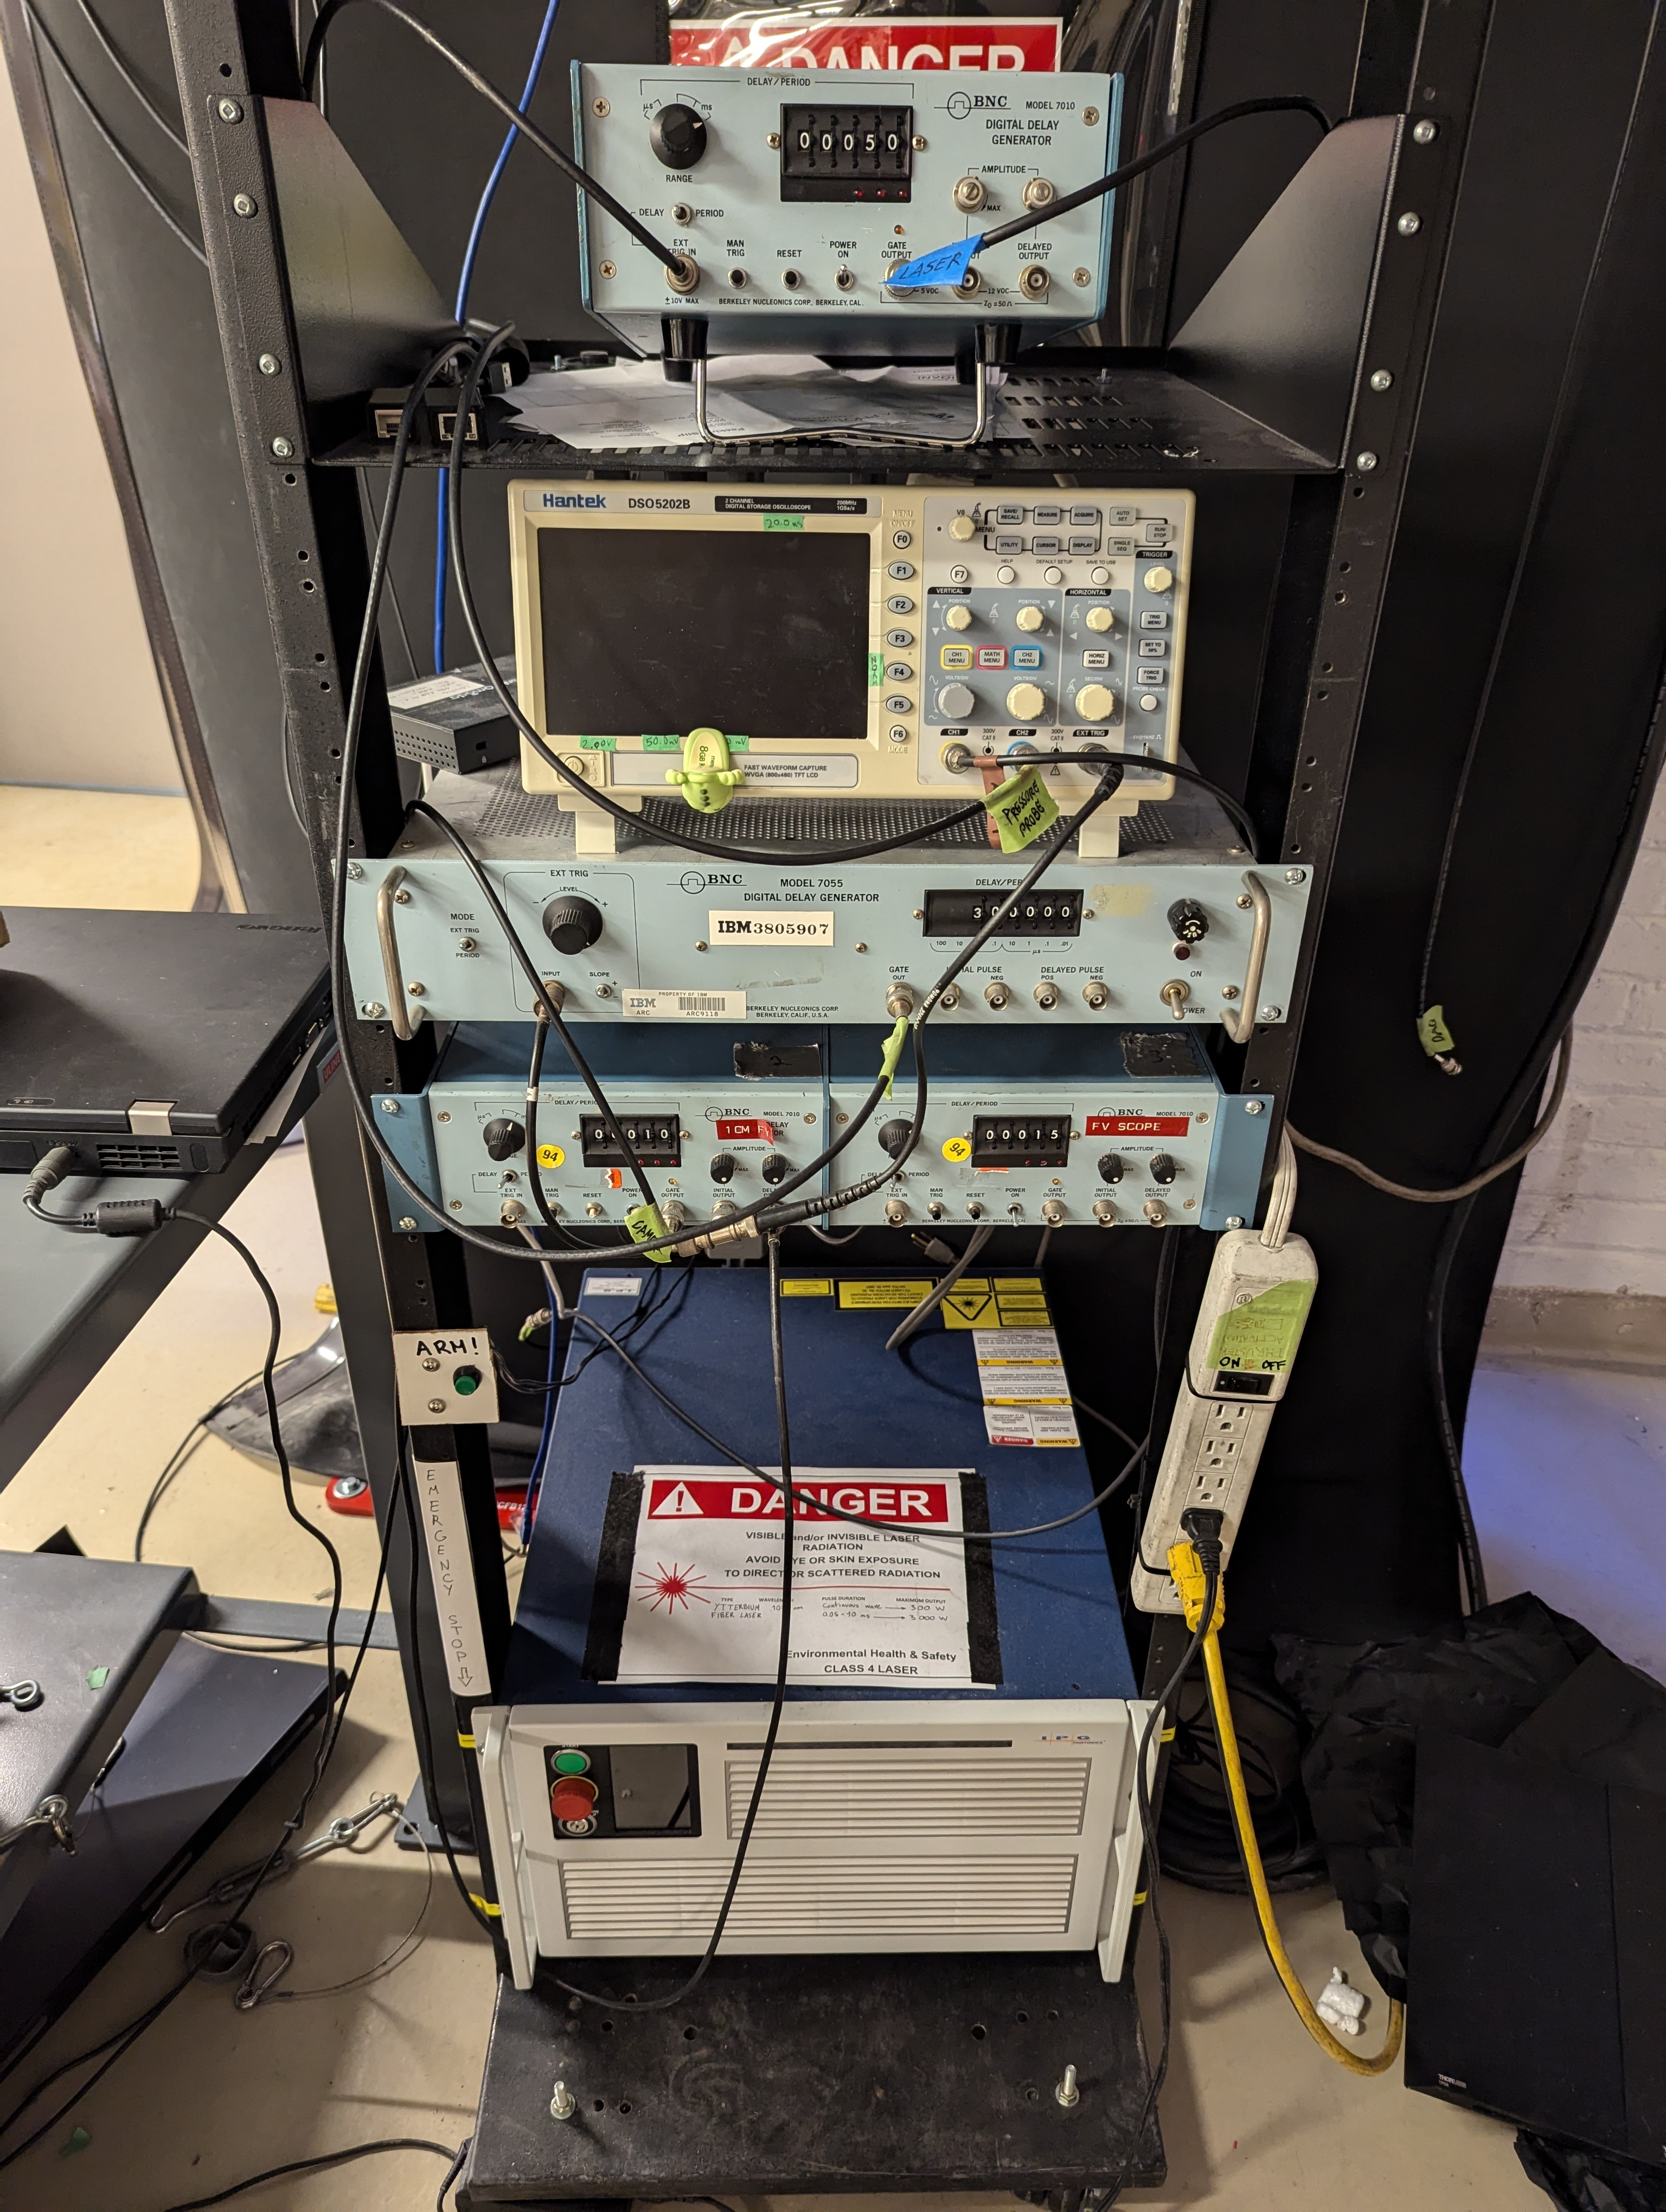
\includegraphics[width=0.50\textwidth]{assets/3 design/Control rack.jpg}
                \caption{Electronics rack with laser at the base}
                \label{fig:electronics rack}
            \end{figure}

            V2 uses two lenses placed close to each other to focus the laser from the collimator. These are the Thorlabs LA1380-C and LA1417-C N-BK7 plano-convex lenses with a \qtyrange{1050}{1700}{nm} anti-reflective coating. Their focal lengths of \qty{500}{mm} and \qty{150}{mm}, respectively, give a combined focal length of \qty{115}{mm}. These two lenses are mounted in a single Thorlabs LMR2 lens mount with two retaining rings. A Thorlabs DT12 translation stage enables left/right alignment of the laser focus, while a Thorlabs DTS25 translation stage gives control on the depth (axial position) of the focus.

        \subsection{Timing control}

            Correct timing of the laser and spark initiation is necessary to initiate LSP. To this end, delay generators are used (BNC models 7010 and 7055) as seen in \autoref{fig:timing section and oscilloscope}. They are mounted at the top of the electronics rack.

            \begin{figure}[!ht]
                \centering
                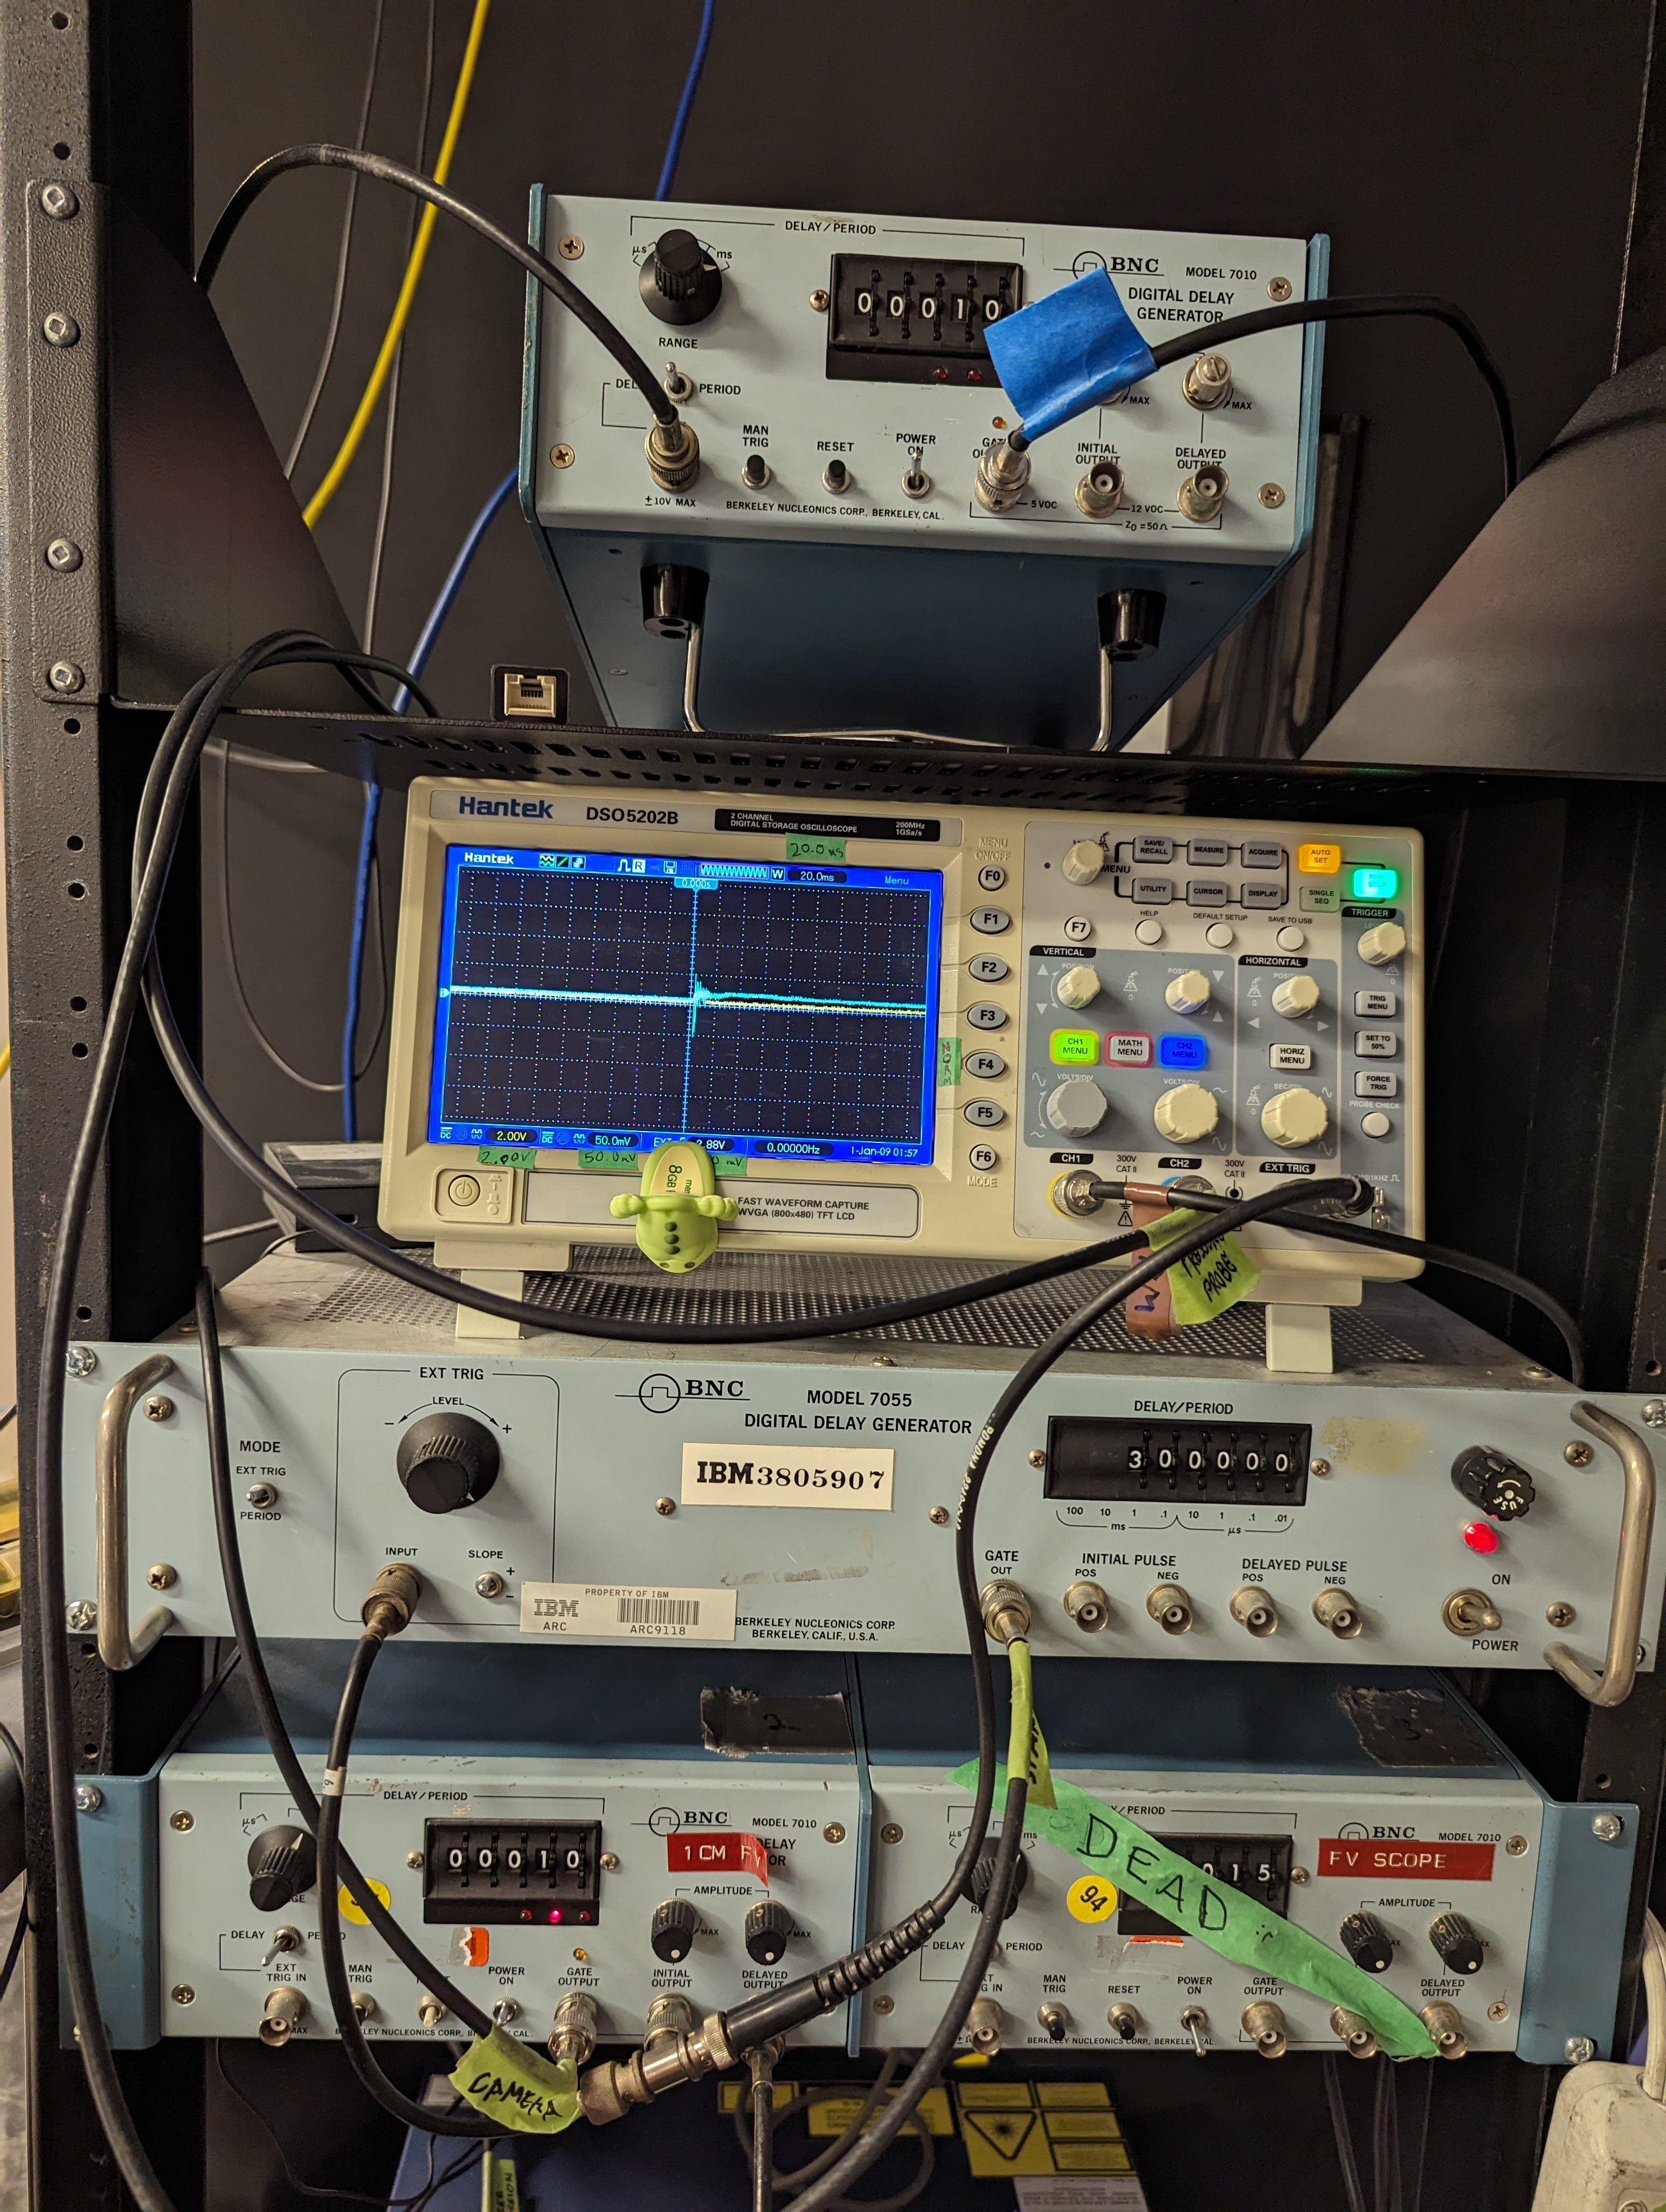
\includegraphics[width=0.50\textwidth]{assets/3 design/Timing rack and oscilloscope.jpg}
                \caption{Delay generators and oscilloscope}
                \label{fig:timing section and oscilloscope}
            \end{figure} 

        \subsection{Data acquisition (DAQ) system and oscilloscope}

            Load cell and pressure transducer voltage is sent to a DATAQ Instruments DI-2018, on \autoref{fig:DAQ}. This data is streamed to a personal computer by USB, where the thrust and pressure traces can be saved for analysis. Two pressure sensors were used: a PCB Model 113B28 and an Omega PX119A-1KG5V. Refer to \autoref{chp:omega calibration} for the Omega pressure sensor calibration.

            \begin{figure}[!ht]
                \centering
                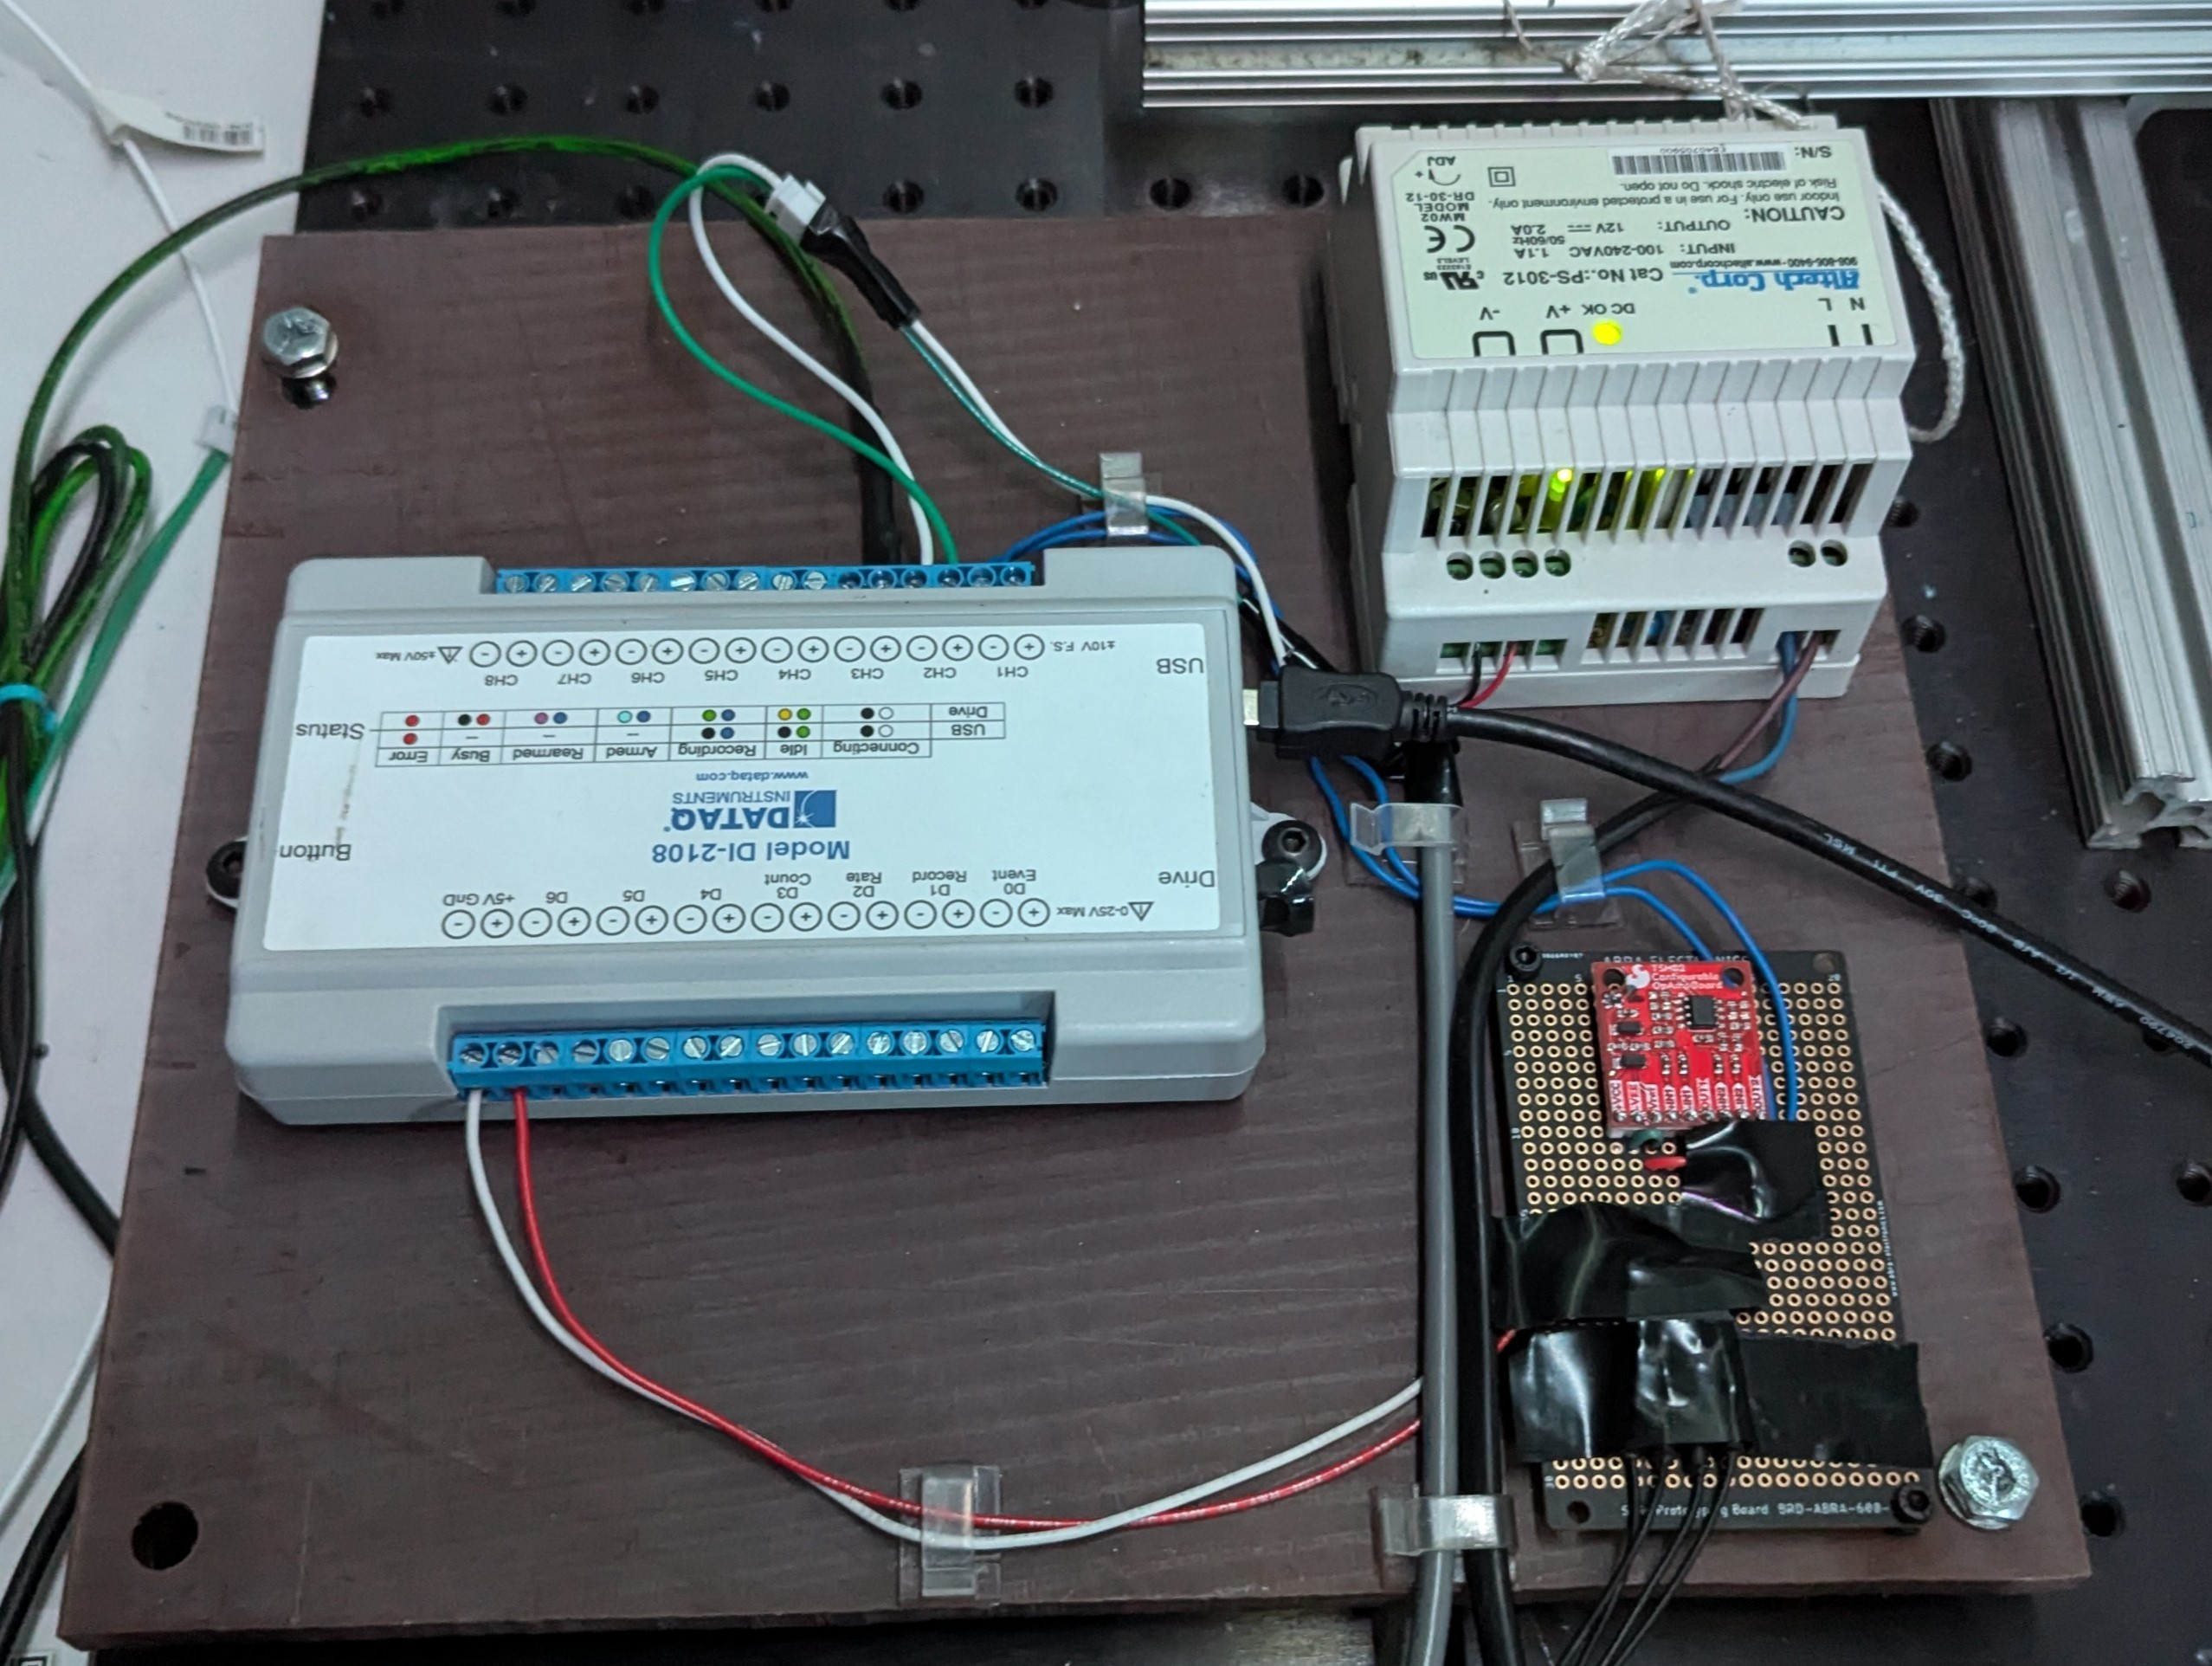
\includegraphics[width=0.50\textwidth]{assets/3 design/DAQ electronics.jpg}
                \caption{DAQ system}
                \label{fig:DAQ}
            \end{figure}

        \subsection{Cameras}

            A Photron SA5 high speed camera was used during certain LSP shots to determine if LSP initiation had happened and how long the plasma had lasted. Due to no side windows being present on V2, the Photron camera looked at an angle from the side into the front window, seeing the reflection of the plasma core (as in \autoref{fig:V2 setup}). During LSP shots, the camera's sensor was protected by an Aurora PowerXND-II Variable Neutral Density Filter and a Hoya \qty{58}{mm} UV and IR cut filter.

            A generic USB webcam was also connected to the data acquisition laptop, giving a live wide-angle view of the entire experiment. As these cameras are sensitive to IR, it gave an extra confirmation that the laser emission was off before opening the laser safety curtain.

        \subsection{Spark initiation system}

            The spark was generated by an AEM 30-2853 High Output Smart Coil, supplied by a \qty{10}{A} power supply. The coil can generate a \qty{40}{kV}, \qty{103}{mJ} spark. The trigger signal wire from the delay generator comes in from the left of \autoref{fig:Spark initiation}. It passes through the power supply electrical box in a quad shielded coaxial cable. The smart coil is placed in a separate electrical box to reduce electromagnetic interference. The spark energy exits through the cable on the right of \autoref{fig:Spark initiation}. 

            \begin{figure}[!ht]
                \centering
                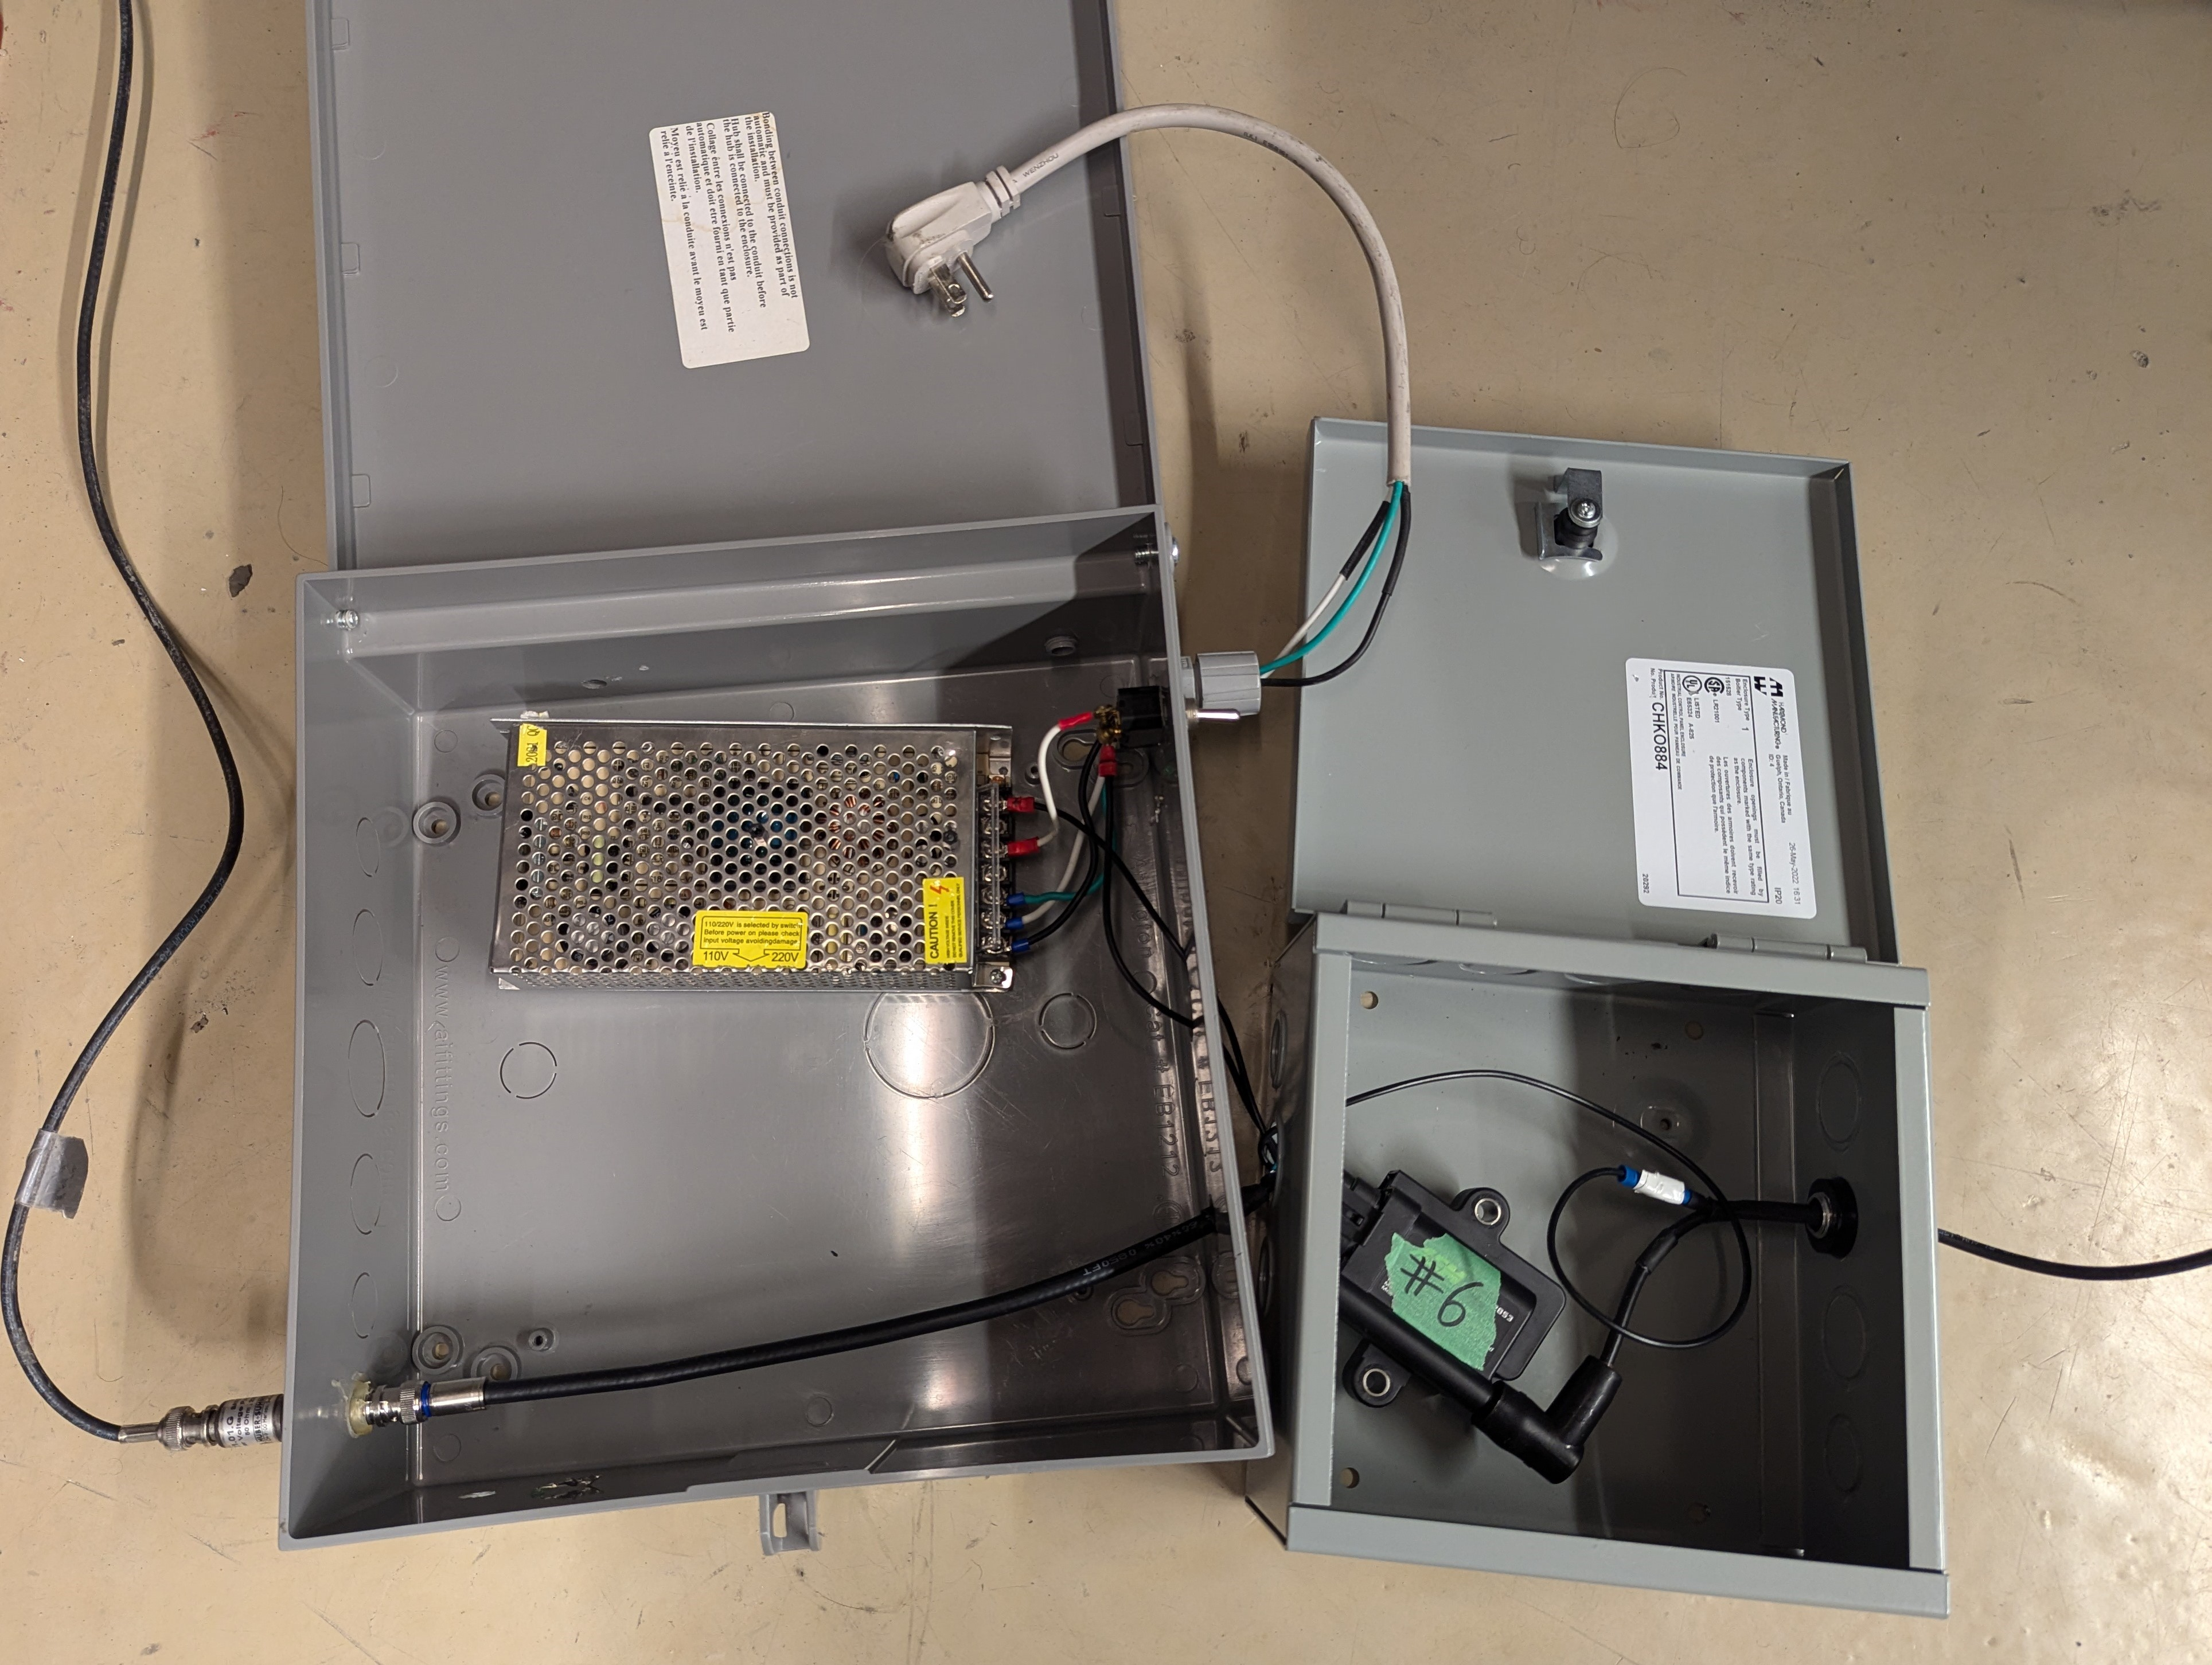
\includegraphics[width=0.50\textwidth]{assets/3 design/Spark initiation system.jpg}
                \caption{Spark initiation system. On the left is a power supply, while spark coil number 6 is on the right.}
                \label{fig:Spark initiation}
            \end{figure}

            \autoref{fig:Assembled electrode design} shows the assembled electrodes, the sharper one being connected to the smart coil's output. The other electrode is grounded.

            \begin{figure}[!ht]
                \centering
                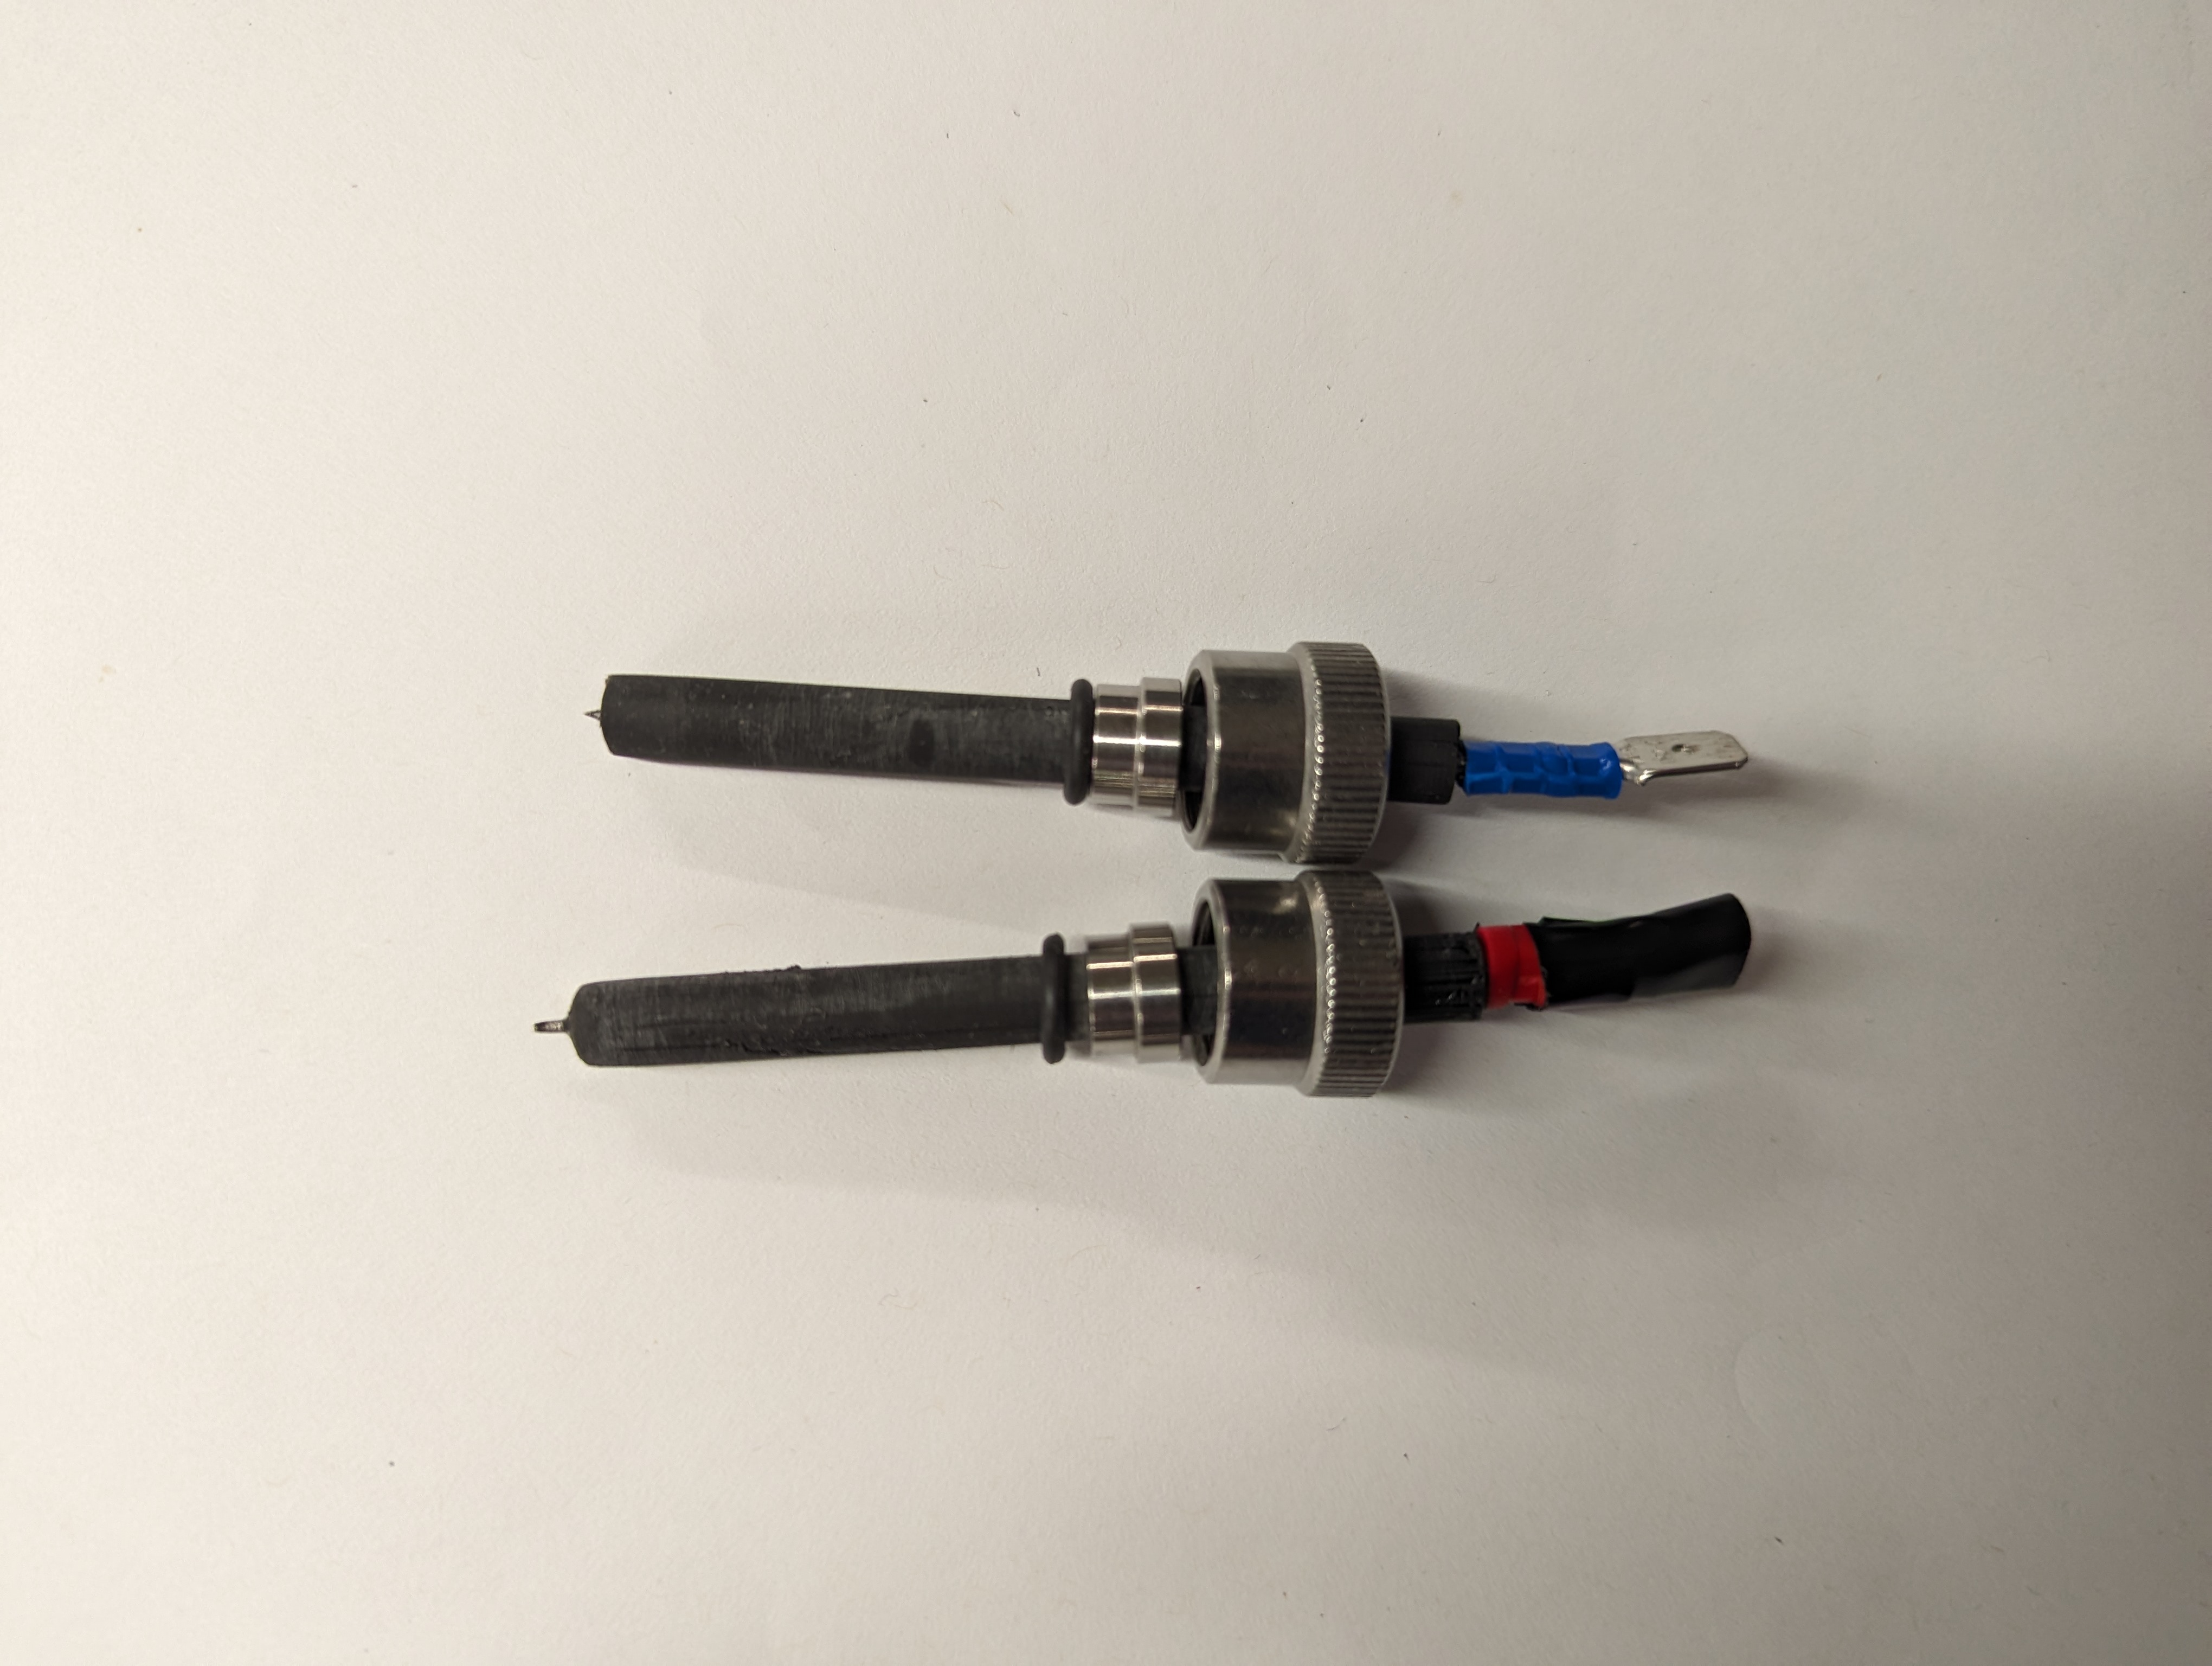
\includegraphics[width=0.5\textwidth]{assets/3 design/V2 electrodes.jpg}
                \caption{Assembled electrodes with Ultra-Torr cap and electrical connectors}
                \label{fig:Assembled electrode design}
            \end{figure}

        \subsection{Needle valve}
            
            To be able to run the thruster in the double choked configuration, an adjustable orifice upstream of the thruster is required. The WL14H-320P needle valve (\autoref{fig:Needle valve}) was chosen for this.

            \begin{figure}[!ht]
                \centering
                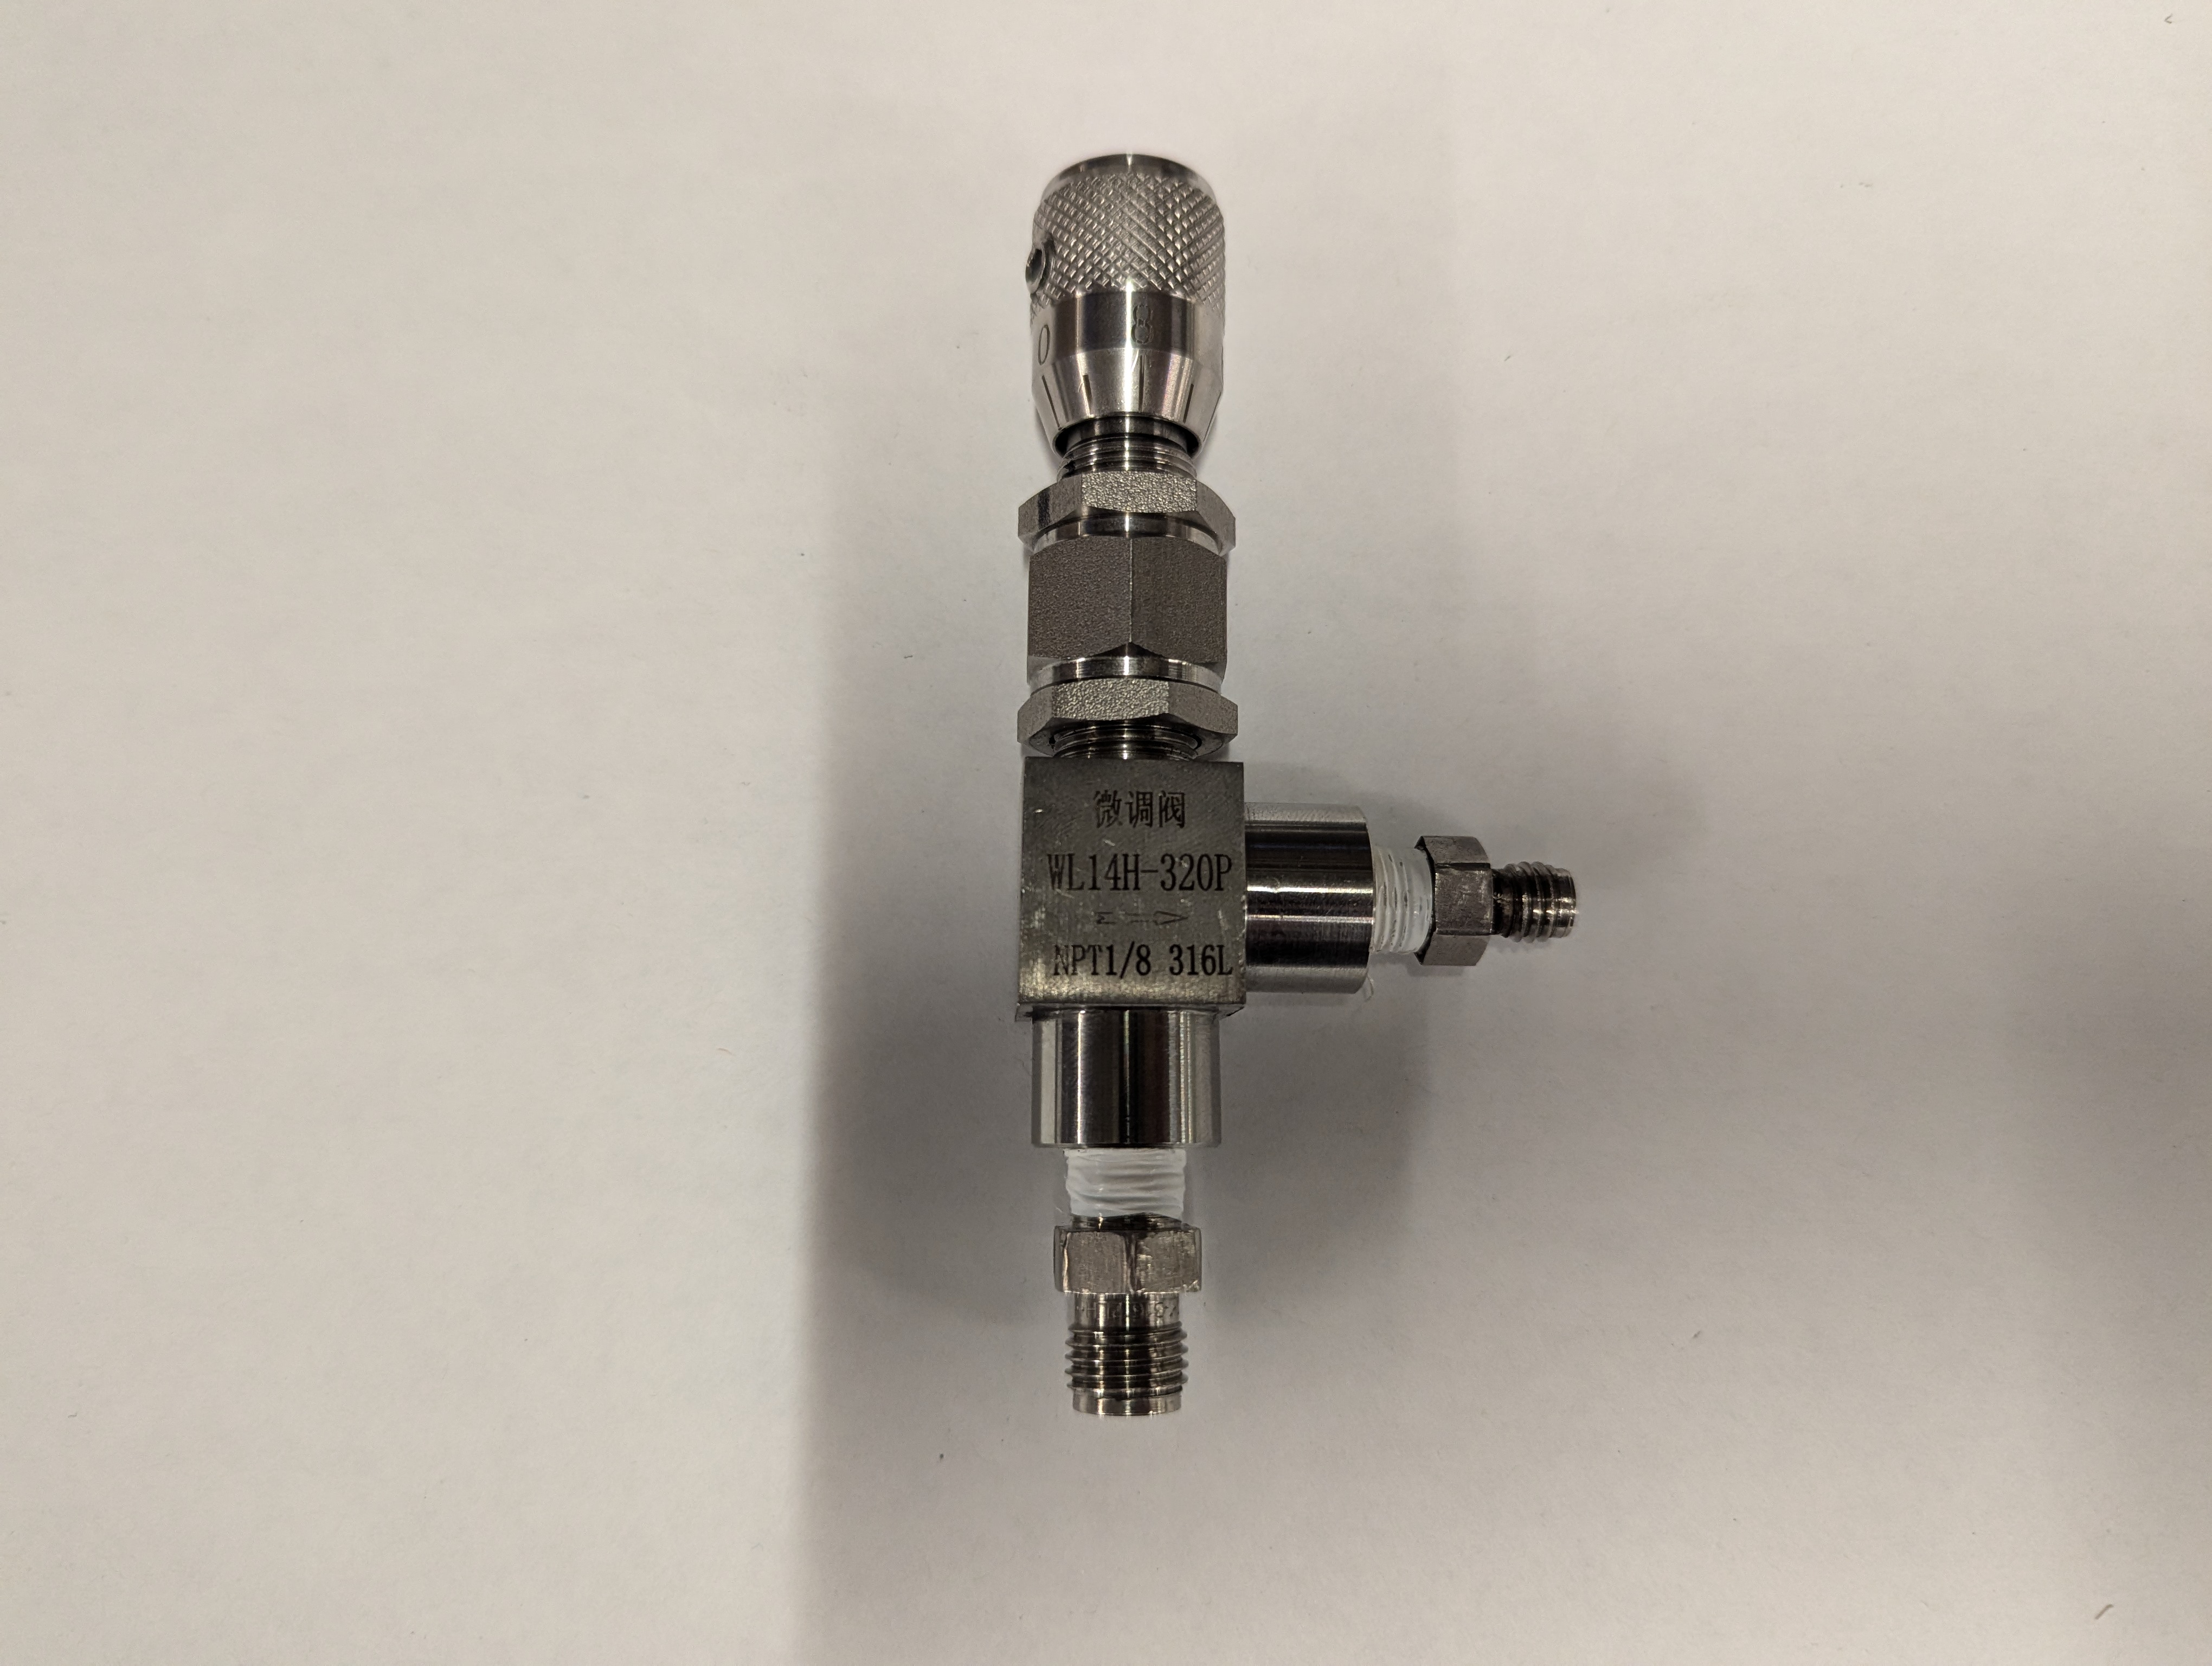
\includegraphics[width=0.50\textwidth]{assets/3 design/Needle valve.jpg}
                \caption{WL14H-320P Needle valve}
                \label{fig:Needle valve}
            \end{figure}

        \begin{figure}[!ht]
            \centering
            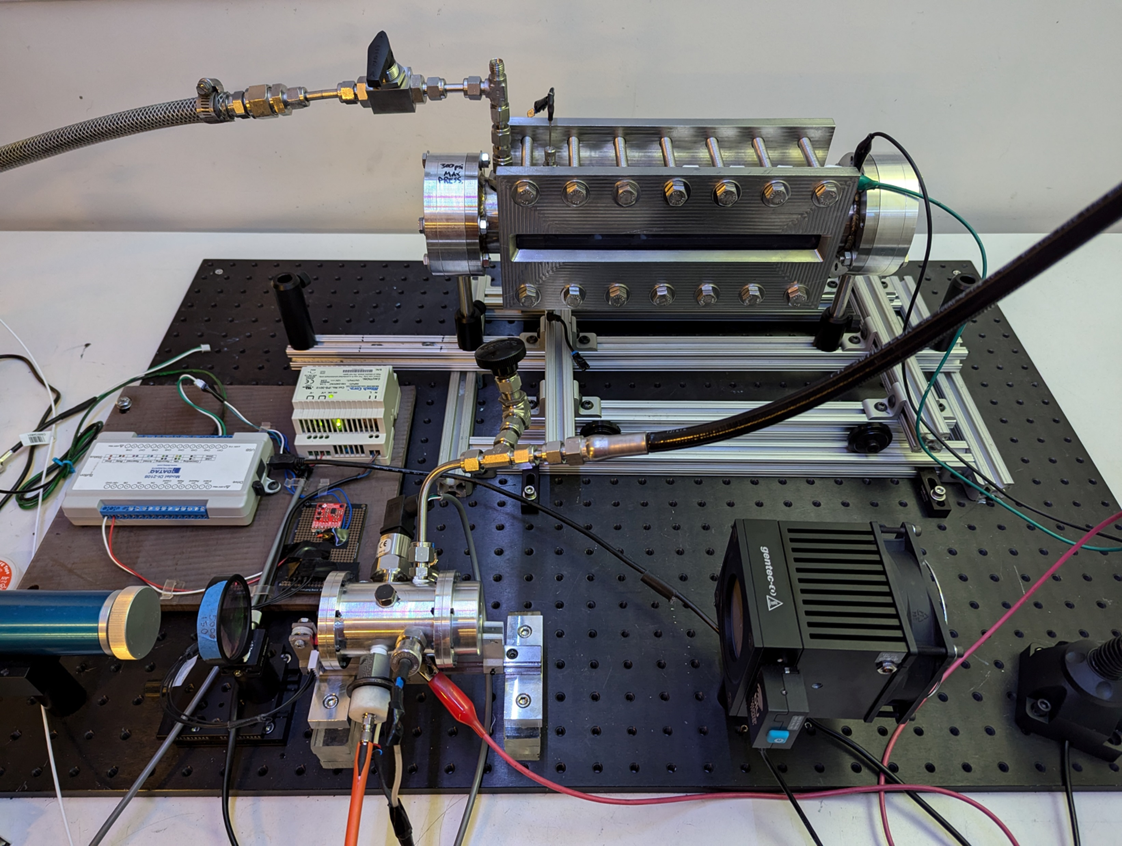
\includegraphics[width=\textwidth]{assets/3 design/V1 V2 comparison.png}
            \caption{Size comparison between V1 (top) and V2 (bottom). V2 is in static configuration, without the extension cylinder.}
        \end{figure} 